\chapter{A Study of the Morphology of the SiII \texorpdfstring{$\lambda$}{}6355 Feature in SNe Ia}
\label{chap:si_feat_pca}

\section{Overview}
\label{intro}
% Type Ia supernovae (SNe Ia) played a key role in the discovery of the accelerating expansion of the universe \citep{perlmutter_measurements_1999, riess_observational_1998}, and continue to be one of the best tools for measuring cosmological distances. Their use as cosmological distance indicators stems from the numerous empirical correlations between observable features of the supernova and their intrinsic brightnesses. The standardization relations used by the most recent supernova cosmology analyses make use of the both correlations between the maximum brightness and the decline rate of the light curve, known as the "Phillips relation" \citep{phillips_absolute_1993}, and correlations between the color of the supernova and the intrinsic brightness \citep{riess_precise_1996, tripp_two-parameter_1998, guy_salt_2005, guy_salt2_2007}. Assuming a linear relationship between supernova decline rate, color, and intrinsic luminosity, SN Ia brightnesses can be standardized to about 0.15 mag \citep{betoule_improved_2014}.

A number of spectroscopic techniques have been shown to improve supernova standardization. The spectroscopic twinning technique presented in \citet{fakhouri_improving_2015} and the twins embedding technique of \citet{boone_twins_2020a} and \citet{boone_twins_2020b} all show that the use of additional spectroscopic information can reduce the scatter in standardized magnitudes beyond the limit of photometric methods using only a single spectrum near maximum brightness. The extended spectrotemporal model SNEMO \citep{saunders_snemo_2018} has also been shown to improve the spread in standardized magnitudes by capturing a wider array of supernova behavior through a more flexible model. \citet{zheng_empirical_2018} combines spectroscopic and photometric measurements to relate the rise time of the light curve and the photospheric velocity measured from a near-maximum spectrum to the peak magnitude of SNe Ia, and found a reduced dispersion in standardized magnitudes among normal velocity objects. Additionally, a number of subclassifications of SNe Ia based on their near-maximum brightness ejecta velocities, ejecta velocity time gradients, and equivalent widths of various spectral features have been introduced in the literature \citep{branch_comparative_2006, benetti_diversity_2005, wang_improved_2009, wang_evidence_2013}. By splitting the supernovae into subgroups based on these spectral indicators, these studies have shown that the scatter in the intrinsic luminosities can be reduced. These studies all use one of the most prominent features of Type Ia supernovae spectra (indeed what separates Type Ia's from other Type I supernovae): the \siliconii{} feature, found at a rest-frame wavelength of about 6150\,\AA. 

In addition to improving standardization, spectroscopy of the \siliconii{} region can be used to detect and probe systematic biases stemming from population drifts with redshift. As an example, we can take the empirical correlation between supernova ejecta velocity measured from the \siliconii{} line and intrinsic color that has been studied extensively \citep{wang_improved_2009, foley_measuring_2011, foley_velocity_2011,foley_relation_2012,mandel_type_2014}. Because of this correlation, uncertainties in velocity propagate into uncertainties in intrinsic color, which themselves propagate to uncertainties in distance modulus. If the distribution of velocities changes with redshift, this effect will lead to a bias when determining cosmological parameters.

While \citet{foley_relation_2012} found no significant difference in the distribution of silicon ejecta velocities between samples at low redshift and samples at somewhat higher redshifts ($ 0.1 <  z  < 0.4$), the author warns that ``the high-redshift samples are still small, and even a small offset could affect cosmological measurements."  Future supernova surveys, like the Nancy Grace Roman Space Telescope supernova survey, will probe redshifts that are much higher than this previous work, and represent very different host galaxy age populations. Correlations between ejecta velocity and host-galaxy mass \citep{foley_relation_2012} and age and metallicity \citep{wang_evidence_2013} suggest the possibility of a redshift evolution in ejecta velocity tied to these drifts in SN environments. In order to avoid these potential biases, it is imperative that we be able to measure the ejecta velocities of the supernovae in future surveys.

Typically, measuring any spectral indicator (i.e. velocities and equivalent widths) involves smoothing the spectrum to remove high-frequency noise and then removing some estimate of the continuum. The equivalent width of the line is obtained by integrating the measurements of the smoothed and continuum-divided spectrum in the region of interest, and the velocity of the line is determined from the blue shift of the wavelength of the minimum of the feature in the wavelength range of interest. The smoothing and minimum-finding method is very effective for spectral observations with high resolution and signal-to-noise, but exhibits some problems when the spectra have lower resolution or higher noise levels. One way of avoiding these types of errors is to assume some parametric form of the spectral feature shape (e.g. a Gaussian), but these parametric shapes often bias the results, as we will see.

In this chapter, we present a new method for reconstructing the velocity and equivalent width of the \siliconii{} feature of Type Ia supernova from low-resolution, noisy spectra that is more robust and less susceptible to bias. This method does not use the smoothing and interpolation techniques that can be problematic in the low-resolution regime, nor does it model the feature with mathematically convenient but physically unmotivated functional forms. Instead, the reconstruction is based on the available data, encapsulating much more of the morphological variation than a simple model would allow, without needing more expensive high-resolution observations. The recovered velocities and equivalent widths can be used with the previously mentioned improved standardization techniques, as well as to correct for possible redshift drift biases.

The chapter is structured as follows: the data used in this analysis is described in Section \ref{data}. In Section \ref{spectral_features}, we discuss the current measurement methods available for modeling the silicon absorption feature in medium- and high-resolution spectroscopy. Section \ref{method} explains our new method, and Section \ref{validation} shows the results of this measurement method on an external validation set \citep[BSNIP,][]{silverman_berkeley_2012}. Section \ref{wfirst} evaluates the method on a simulated data set of supernovae at high-redshift observed with the proposed Roman Space Telescope prism. We conclude in Section \ref{conclusions}.

\section{Data}
\label{data}
The spectra used in the training set were obtained with the Supernova Integral Field Spectrograph \citep[SNIFS,][]{lantz_snifs_2004} mounted on  the south-bent Cassegrain port of the University of Hawai`i 2.2m telescope, operated remotely by members of the Nearby Supernova Factory collaboration \citep[SNfactory,][]{aldering_overview_2002}. The SNIFS integral field spectrograph uses lenslet arrays to divide its 6$''$ x 6$''$ field-of-view into a grid of 15 x 15 spatial elements (spaxels). Each spaxel is fed into a dual-channel spectrograph that covers 3200-5200\,\AA{} in the blue and 5100-10,000\,\AA{} in the red, with a spectral resolution of $R \sim 1000$. The data from this instrument was reduced using our dedicated pipeline, detailed in Ponder et al. (in preparation).

The SNfactory supernova sample\footnote{This analysis is based on the \texttt{ALLEG2a} internal production from the data reduction pipeline.} contains 275 objects with at least 5 spectral observations. These 275 objects have a total of 3731 spectro-photometric observations, with each object having an average of 13-14 spectral observations. The sample is subdivided into ``good," ``bad" and ``auxiliary" subsamples based on SALT2 light curve fits to synthesized photometry and spectral classification. All objects in the ``good" category meet the following criteria:
\begin{itemize}
    \item At least 5 total observations
    \item One epoch within -10 and +7 days of maximum brightness based on SALT2 fits to light curves generated through synthetic photometry
    \item 4 epochs between -10 and +35 days of maximum brightness 
\end{itemize}
These quality cuts ensure that the supernova time series are detailed enough to properly constrain the light curve model parameters, particularly the time of maximum brightness. There are 223 objects in this ``good" subsample, which we take as our full training set. Each of the spectra in this data set has been corrected for Milky Way dust reddening and shifted in wavelength to a redshift of $z=0$. The overall flux has also been normalized so that each spectrum's flux is as it would be if the supernova were located at a redshift of $z=0.05$, assuming a fiducial flat $\Lambda$CDM cosmology with $H_0=70$~km/s/Mpc and $\Omega_m = 0.3$.

Our focus is on spectra near maximum brightness. Thus, we restrict the training set to those spectra observed within $\pm 2$ rest-frame days of maximum light (as determined from SALT2.4 fits to the synthesized light curves). A total of 241 spectra from 163 objects meet this criterion, 127 spectra from 86 supernovae in the training subsample and 114 spectra from 77 supernovae in the validation subsample. When a single supernova has many observations within $\pm 2$ days, we use the observation closest to maximum light. The $\pm 2$ day window ensures that we can capture more supernovae into our training sample while also ensuring that the deviations from the maximal brightness spectrum are small.

Our analysis is also only focused on the relative sizes and shapes of the spectral features, and the overall flux and color calibration is irrelevant. To normalize the data, we divide the spectrum by a spline fit to each spectrum with 13 evenly spaced knots from 2500~\,\AA{} to 10,000~\,\AA{}. This is the same normalization performed by the Supernova Identification code \citep[SNID,][]{blondin_determining_2007} and is performed to remove the effects of differential dust reddening in our line profile models. In Figure \ref{spline_norm_ex}, we show an example of this spline fit and in Figure \ref{compare_spline_norm}, we show what the \siliconii{} feature looks like with and without this normalization. This normalization has potential to affect the determination of the pseudo-continuum (defined later in Section \ref{spectral_features}), but this effect was found to have negligible impact on the measured velocity in our tests. The final spline-normalized spectra in the \siliconii{} region (5600-6600~\,\AA{}) are made available in the code repository corresponding to this work.

\begin{figure}[htbp]
    \centering
    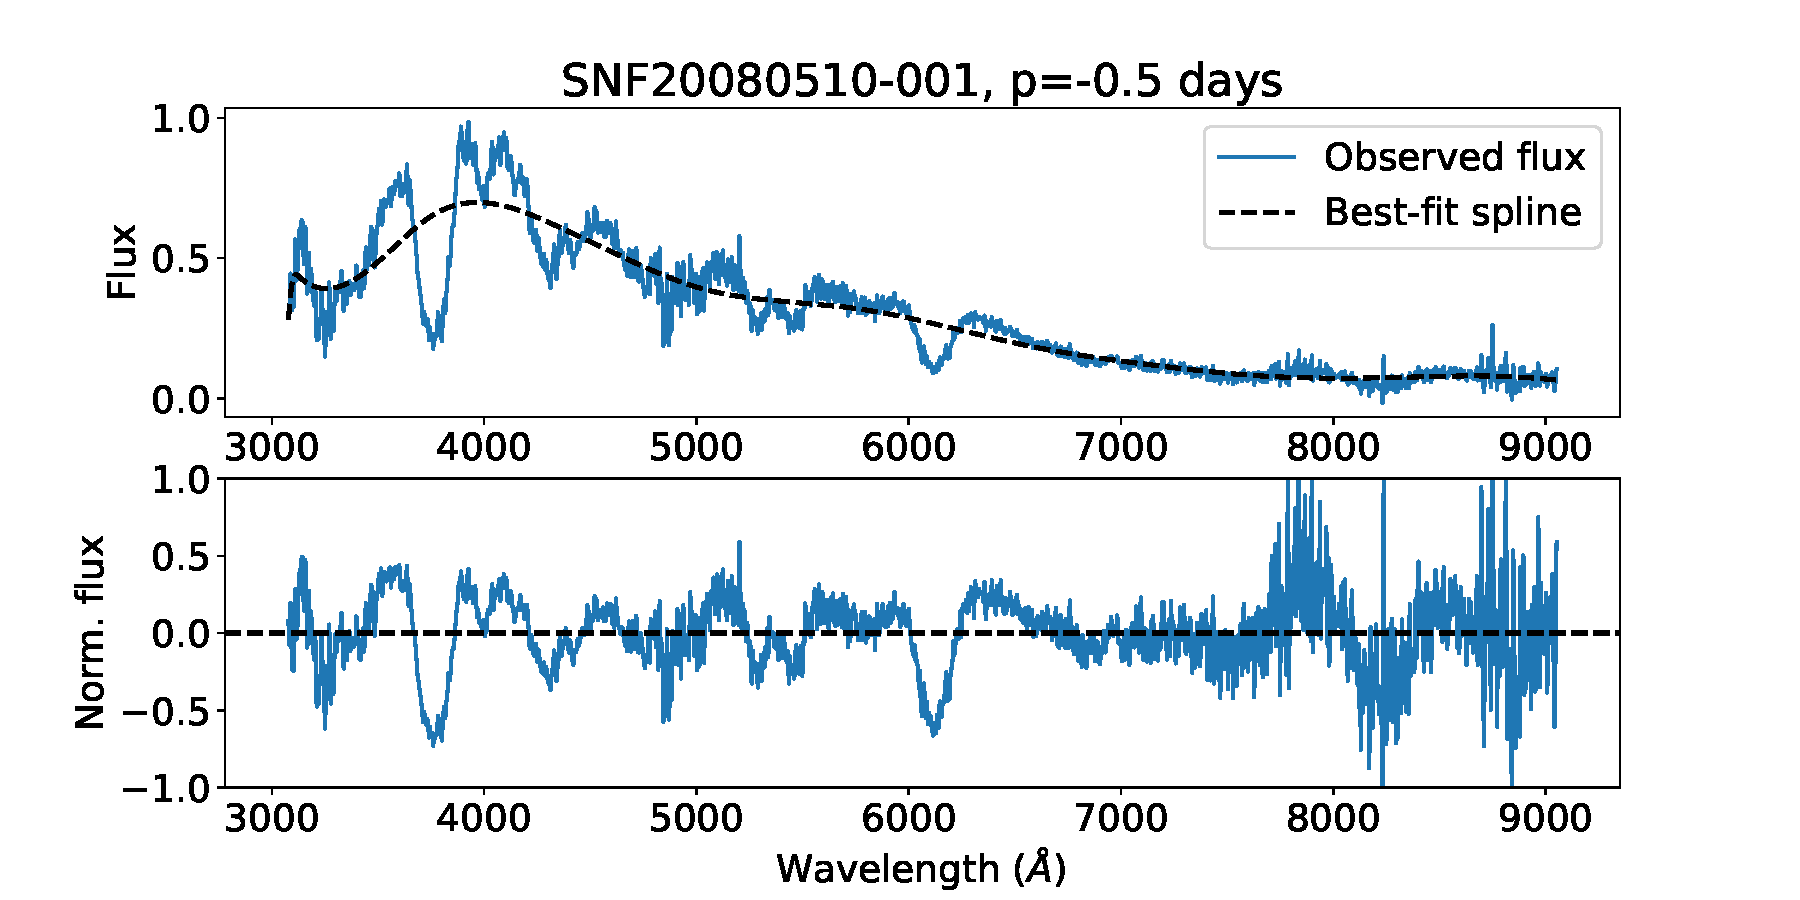
\includegraphics[width=0.9\textwidth]{figures/si_feat_pca/spline_norm_ex.pdf}
    \caption{An example of the preprocessing steps taken to normalize the spectra using a 13-point spline. The upper figure shows the full near-max spectrum along with the best fit spline. The lower figure shows that same spectrum with the spline pseudo-continuum removed.}
    \label{spline_norm_ex}
\end{figure}

\begin{figure}[htbp]
    \centering
    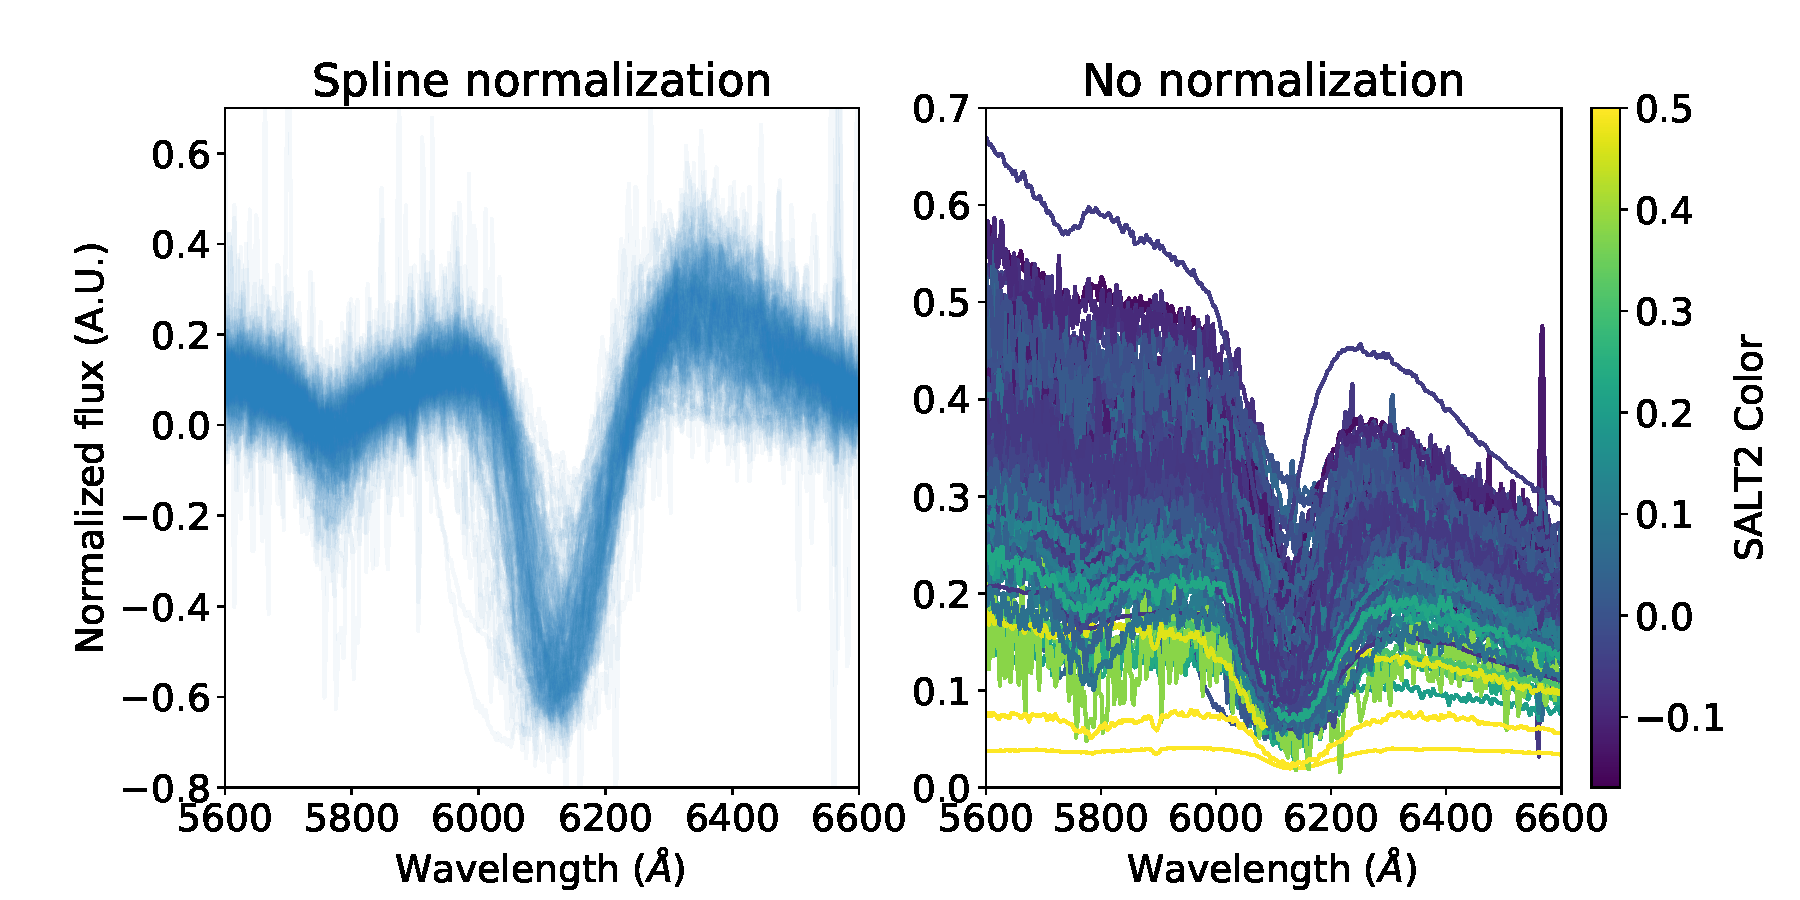
\includegraphics[width=0.9\textwidth]{figures/si_feat_pca/compare_spline_norm.pdf}
    \caption{Zoom-in on the feature of interest for this work, with and without the spline normalization. The features plotted in the right figure are colored by the objects' SALT2 color to emphasize that the effect of this spline normalization is to remove the effects of color on the shape of the spectral feature.}
    \label{compare_spline_norm}
\end{figure}

We also want to ensure that our model generalizes to unseen supernovae by evaluating its performance on an separate test set. This external validation set was taken from the Berkeley Supernova Ia Program \citep[BSNIP,][]{silverman_berkeley_2012}. From the 1298 spectra from 582 objects in this sample, we selected objects with a spectrum within $\pm$3.5 days of maximum brightness and exclude peculiar objects (i.e. those determined to be SN1991T- or SN1999bg-like by SNID). Once again, if one object has more than one spectrum within the phase range allowed, we select the spectrum closest to maximum brightness. This leaves us with a set of 88 spectra. We performed the same preprocessing to these spectra as we did the SNfactory sample spectra. The preprocessed line profiles are also available in the released code repository.

\section{Spectral Feature Measurement}
\label{spectral_features}
As photons from radioactive activity in the inner layers of the supernova explosion make their way through the outer ejecta, they are absorbed by the outer material. This absorption results in the characteristic features in the supernova spectrum. The shape of these absorption lines is governed by myriad physical factors, including the velocity, temperature and density of the ejecta and the optical depth of the various layers of the explosion.

Supernova spectral features profiles are usually quantified using measures of their width and depth, along with their location in the spectrum. The width and depth of the line are summarized by the equivalent width: the width of a rectangle with a height determined by the flux of the continuum such that the area of the rectangle equals the area of the line flux under the continuum. Mathematically, this is
\begin{equation}
    pEW = \displaystyle\int_{\lambda_b}^{\lambda_r}
    \left(1-\frac{f(\lambda)}{f_c(\lambda)}\right)d\lambda,
    \label{equiv_width_eq}
\end{equation}
where $\lambda_b$ and $\lambda_r$ are the wavelength limits of the feature one the blue and red sides, respectively, $f(\lambda)$ is the true flux of the object and $f_c(\lambda)$ is the flux of the continuum.

Calculating the continuum in supernova spectra is challenging, since the absorption features are actually blends of multiple wide lines. Instead, we define a pseudo-continuum by the line connecting the maximum flux values in predefined windows on either side of the absorption feature (see Figure \ref{smooth_example}). These windows are defined in Table \ref{wavelength_ranges}. Throughout the rest of this work, we will use the pseudo-equivalent width, i.e. where $f_c$ in Eq. \ref{equiv_width_eq} is the pseudo-continuum.

\begin{table}[htbp]
    \centering
    \begin{tabular}{cc}\toprule
         Parameter name & Value \\\midrule
         $\lambda_0$ & 6355 \\
         $\lambda_{min}$ & 5600 \\
         $\lambda_{max}$ & 6600 \\
         $\lambda_b$ & 5850-6015 \\
         $\lambda_r$ & 6250-6365 \\\bottomrule
    \end{tabular}
    \caption{Important wavelengths for measuring indicators of the \siliconii{} feature. $\lambda_b$ and $\lambda_r$ are the blue and red windows used when defining the pseudo-continuum.}
    \label{wavelength_ranges}
\end{table}

We can also learn about the ejecta velocities from the location of the absorption feature. We measure the wavelength of maximum absorption $\lambda$ and calculate the velocity using the relativistic Doppler formula:
\begin{equation}
v = c\left[\frac{(\lambda/\lambda_0)^2 -1}{(\lambda/\lambda_0)^2 +1}\right]
\label{doppler}
\end{equation}
where $c$ is the speed of light and $\lambda_0$ is the emission wavelength of the feature (Table \ref{wavelength_ranges}). Because this line is always blue-shifted (the visible ejecta in the line of sight are moving toward the observer), we neglect the minus sign and refer to lines that are more blue-shifted as representing higher velocity ejecta.

\subsection{Baseline: Savitsky-Golay Smoothing}
We begin by establishing a ground truth measurement of the velocities and equivalent widths of all of the supernovae in our training and validation sets. We start by smoothing the spectrum with a Savitsky-Golay filter. The window for this filter is determined optimally as described in Appendix \ref{sg_optimal}. An example smoothed spectrum is shown in Figure \ref{smooth_example}.

Using this smoothed spectrum, we search for the wavelength of maximal absorption (minimum flux) within the window defined by the reddest edge of the blue pseudo-continuum window and the bluest edge of the red pseudo-continuum window and use this wavelength in Eq. \ref{doppler}. We also use the smoothed spectrum to calculate the pseudo-equivalent width with \ref{equiv_width_eq}, where the integration is done with a Riemann sum of the smoothed flux. We estimate our uncertainty on both these measurements using Monte Carlo simulations, repeating the process for spectra with different realizations of the noise. Figure \ref{indicator_scatter_hist} shows the distribution of velocities measured with this technique for all of the supernovae in our training set, and Appendix \ref{app:snf_data_table} contains a table with all the velocity and pseudo-equivalent width measurements, along with their uncertainties. Our training set has a mean velocity of $11.0 \times 10^3$~km/s, with a standard deviation of $1.0 \times 10^3$~km/s. 16.5\% of the objects in the sample are high-velocity (defined as in \cite{wang_evidence_2013} as supernovae with $v_{Si}>12000$~km/s). The distribution pseudo-equivalent widths has a mean of 101~\,\AA{} and standard deviation of 26.2~\,\AA{}.

\begin{figure}[htbp]
    \centering
    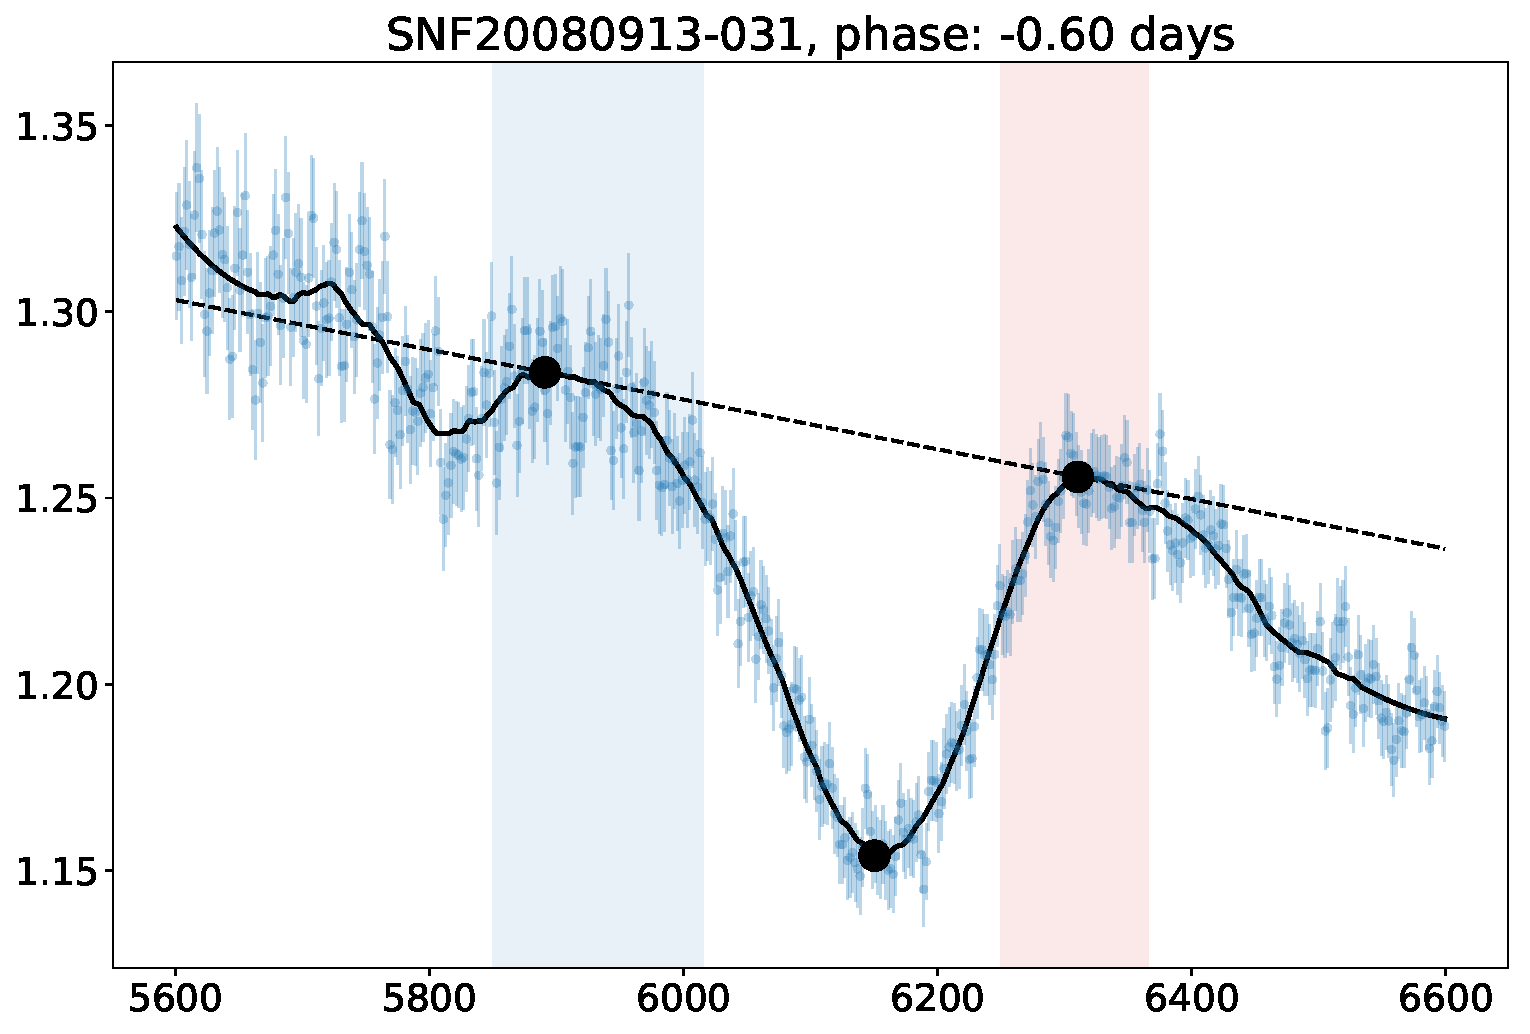
\includegraphics[width=0.9\textwidth]{figures/si_feat_pca/example_measure.pdf}
    \caption{An example \siliconii{} feature. The original data is shown in blue along with the uncertainties. The optimal smoothing is shown in the thick black line. The blue and red spans show the location of the wavelength windows used to search for the maxima defining the pseudo-continuum (the maxima are the large black points). The pseudo-continuum is plotted as the dashed black line. The location of the maximum absorption wavelength is also shown as a large black point.}
    \label{smooth_example}
\end{figure}

\begin{figure}[htbp]
    \centering
    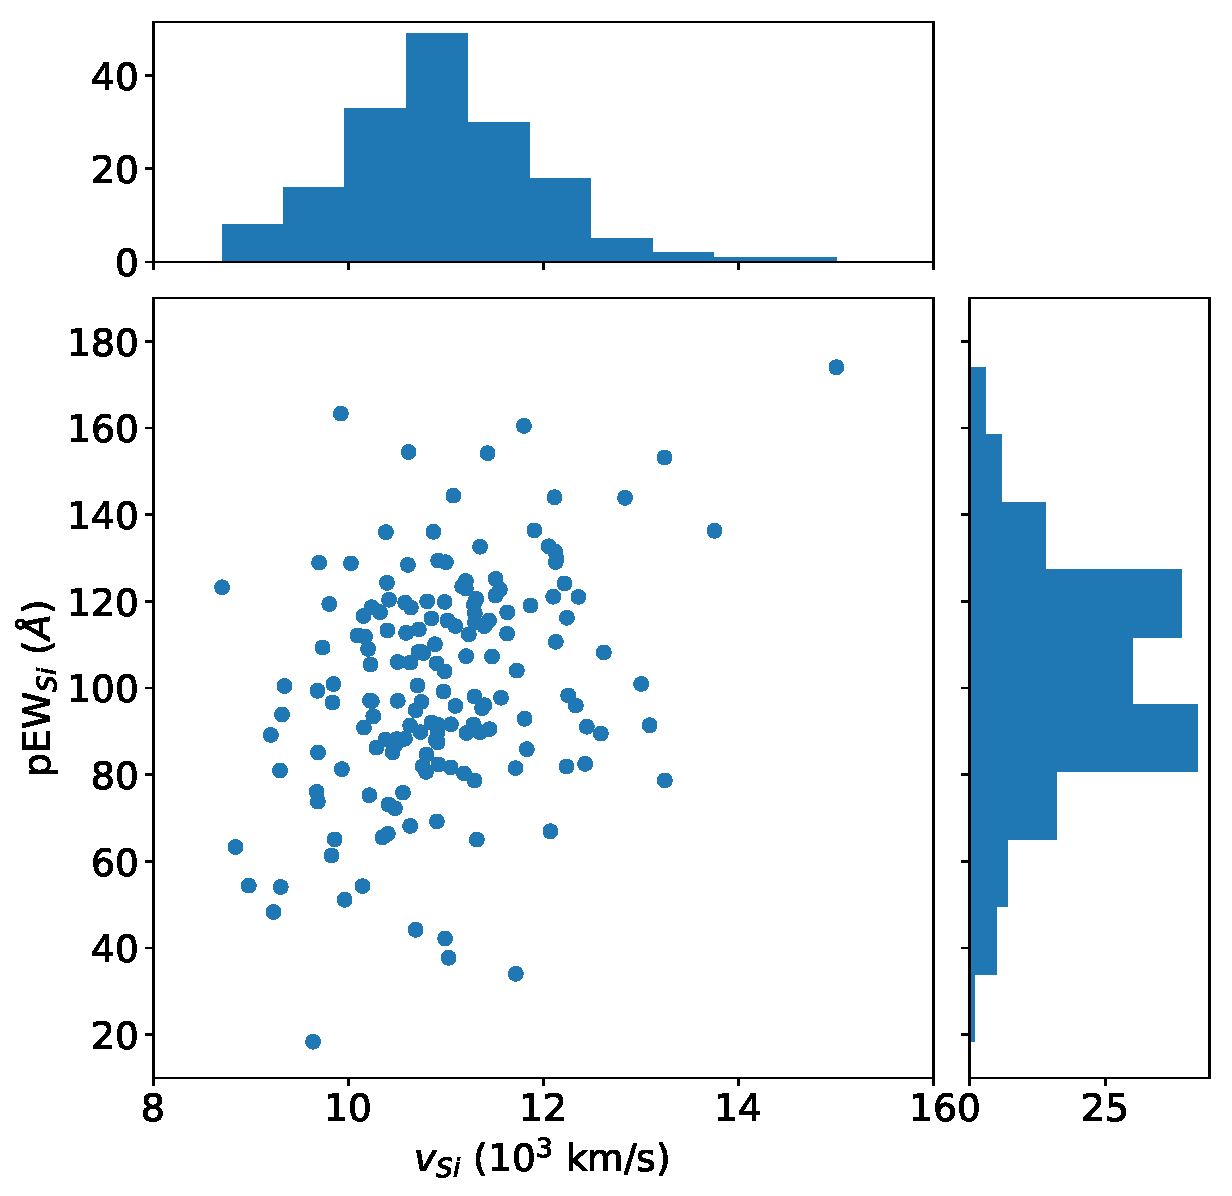
\includegraphics[width=0.9\textwidth]{figures/si_feat_pca/spectral_features_training_scatter_hist.pdf}
    \caption{Distributions of the spectral indicators of the \siliconii{} feature from the training set.}
    \label{indicator_scatter_hist}
\end{figure}

This technique for smoothing the spectrum works very well when the spectrum has reasonable resolution and a high signal-to-noise ratio. However, as the resolution and signal-to-noise level decreases, so too does our ability to recover both the limits of the pseudo-continuum and the true location of maximum absorption. 

\subsection{Gaussian Absorption Line Model}
One way to work around the limitations of low resolution spectroscopy would be to assume some functional form for the absorption feature being studied. A common -- though not very descriptive -- choice is a Gaussian. Using such an inflexible function to capture the line information biases the results. To illustrate this, we fit the same data with a model assuming a linear continuum in the wavelength range of interests along with a Gaussian absorption line. Figure \ref{gauss_feat_fit} shows an example of such a fit. We can see that the full morphology of the feature is not totally captured. More quantitatively, we show in Figure \ref{gauss_bias} a histogram of the difference between the velocity measured from using a Gaussian line profile with a linear continuum and the velocity measured from smoothing and finding the maximum absorption wavelength. There is a clear bias in the velocity; on average, the velocity measured with the Gaussian profile is 200~km/s higher than the true velocity. The pseudo-equivalent width measurements are also slightly biased; on average, the Gaussian measured pEWs are 5~\,\AA{} narrower than the true values.

\begin{figure}
    \centering
    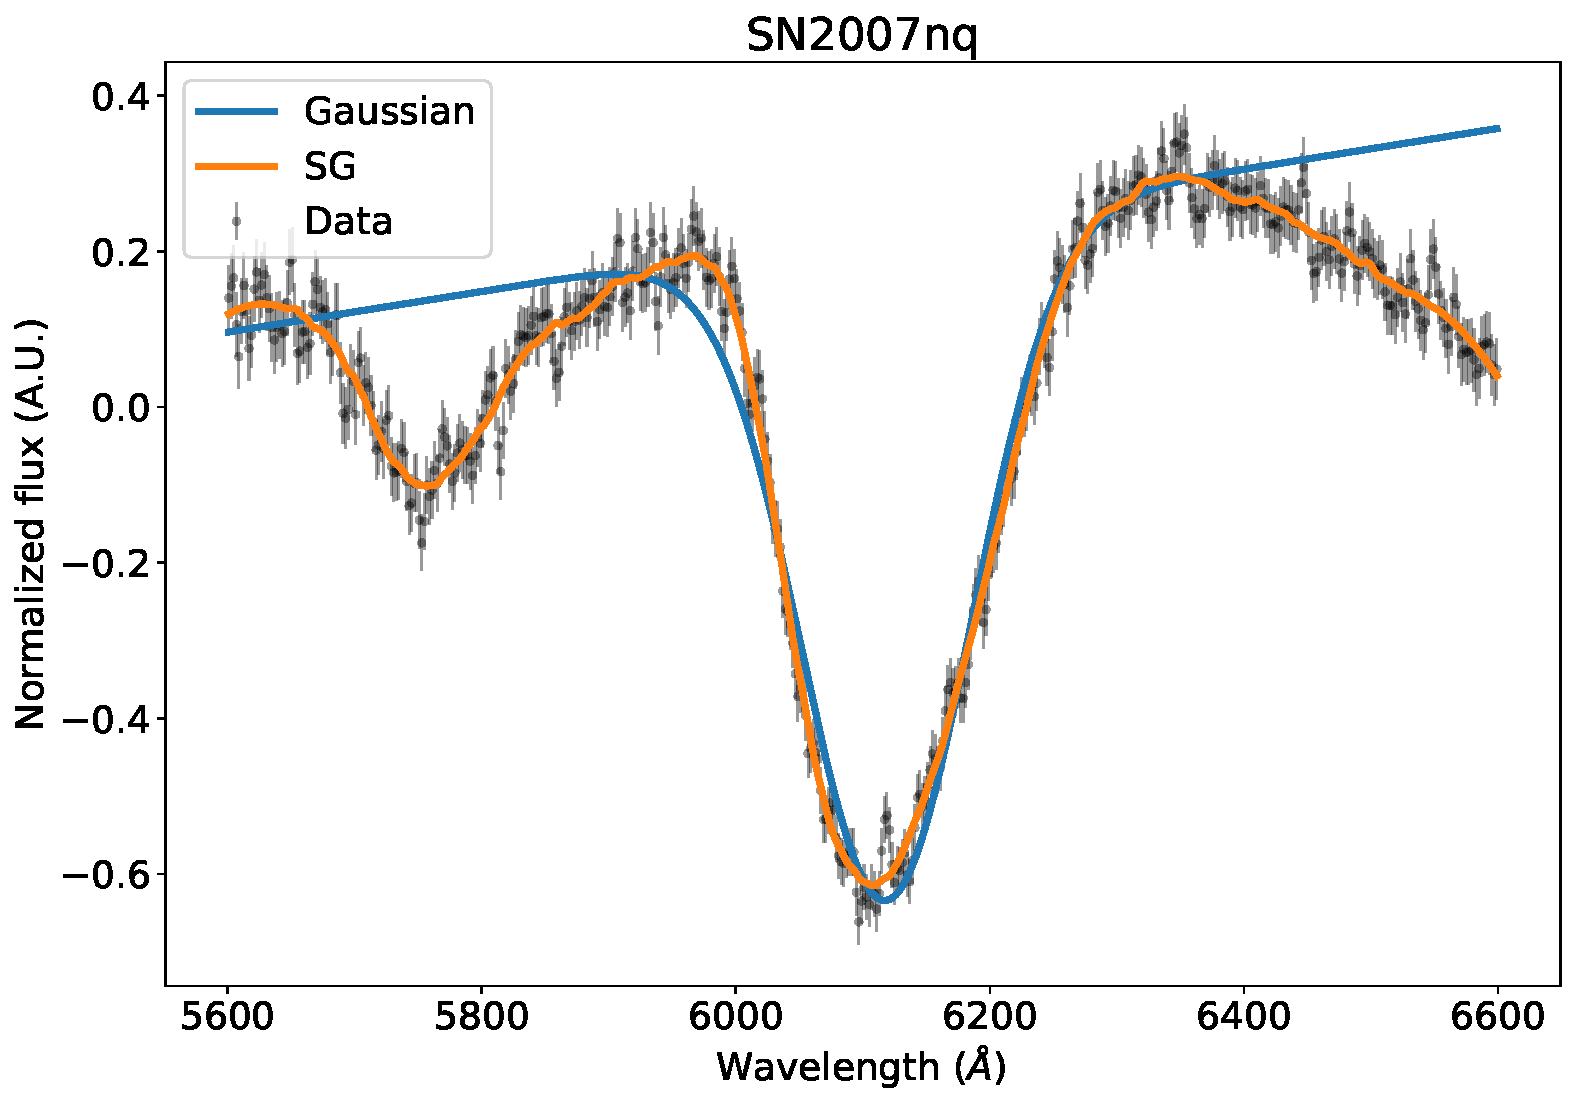
\includegraphics[width=0.9\textwidth]{figures/si_feat_pca/gauss_fit_example.pdf}
    \caption{Comparison of the \siliconii{} feature fit to a Gaussian and the Savitsky-Golay smoothing for SN2007nq. We can see that the blue edge of the feature is not properly captured. The minimum of the feature is also located at different wavelengths, which will produce an inaccurate velocity measurement.}
    \label{gauss_feat_fit}
\end{figure}

\begin{figure}[htbp]
    \centering
    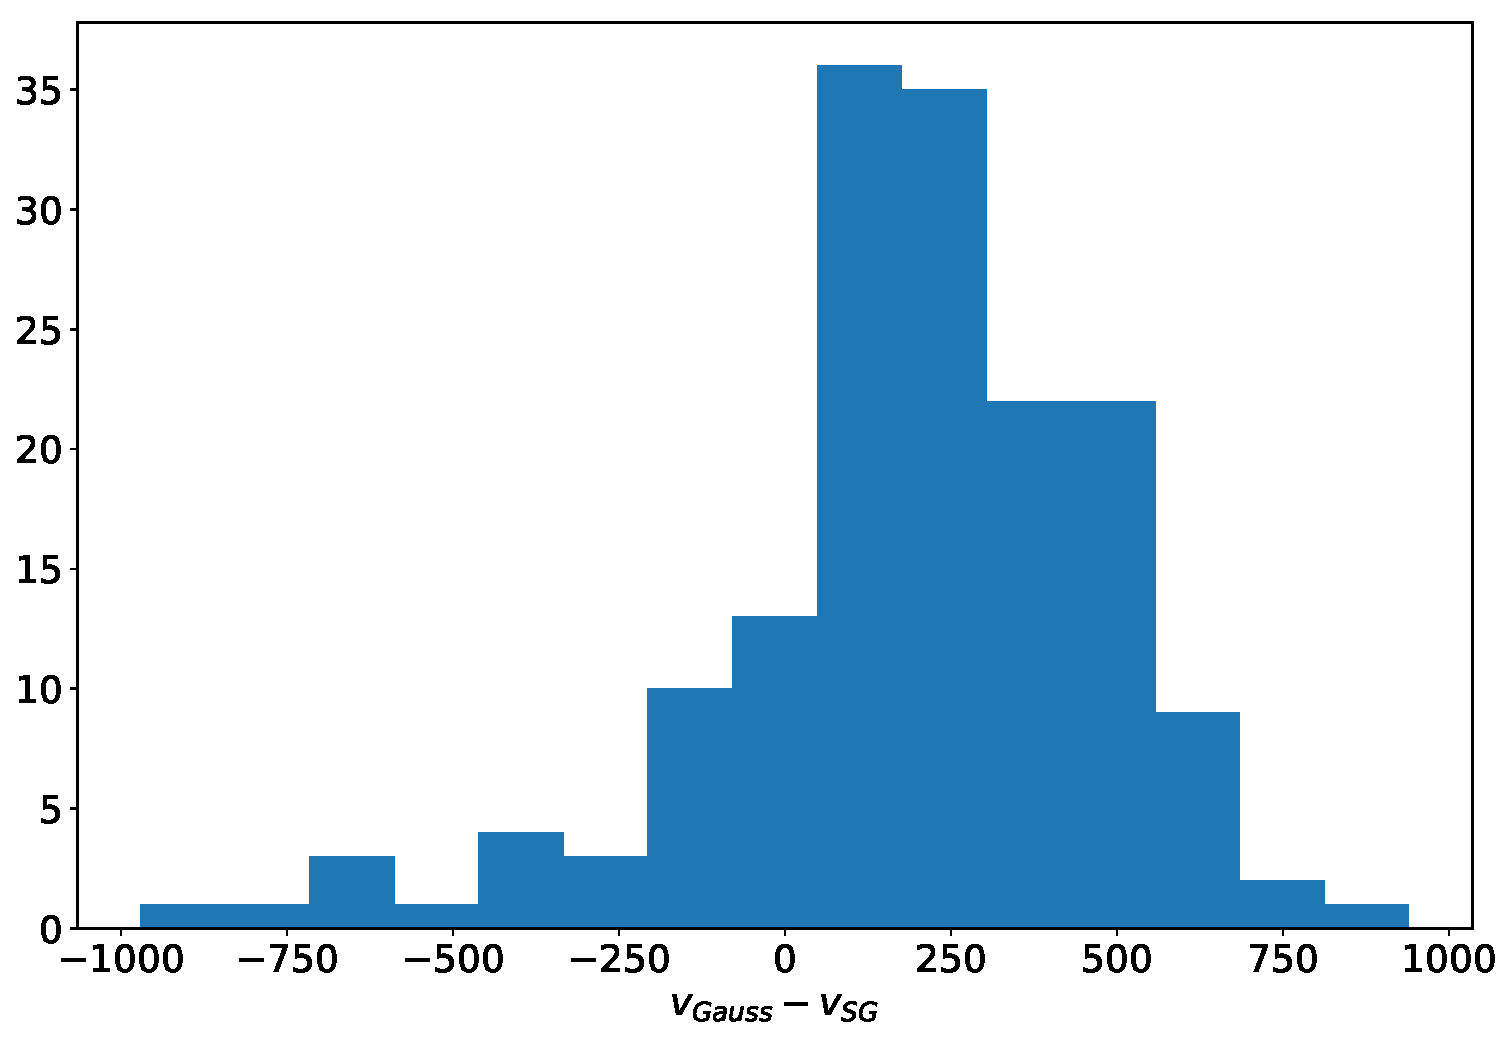
\includegraphics[width=0.9\textwidth]{figures/si_feat_pca/gauss_bias.pdf}
    \caption{Histograms of residuals between the velocity and equivalent width of the \siliconii{} line measured using a Gaussian line profile and the true velocity. There is a clear bias, with the Gaussian measurement giving velocity values that are on average 200~km/s higher than the true values, and equivalent width values that are 5~\,\AA{} narrower.}
    \label{gauss_bias}
\end{figure}


\section{EMFA of the SiII \texorpdfstring{$\lambda$}{}6355 Feature}
\label{method}
Our goal is to introduce a method of inferring the shape of the \siliconii{} feature that is robust to noise and resolution degradation and also accounts for the true diversity of shapes the spectral feature can take on. We accomplish these goals by performing expectation-maximization factor analysis on the normalized spectral features.

\subsection{Expectation Maximization Factor Analysis}
A common unsupervised learning task is dimensionality reduction: using a data set with many features to find a smaller number of principal features that are sufficient to model the data set. The most commonly used technique for dimensionality reduction is principal component analysis, which linearly maps data to a lower-dimensional subspace of the original feature space in such a way as to maximize the data variance. In this analysis, we use a related dimensionality reduction technique: expectation-maximization factor analysis.

Consider a set of $p$ $n$-dimensional data vectors $\{\bm{y}^1, ..., \bm{y}^p\}$. Now assume that there exists some $k$ unobserved latent variables $\{\bm{x}^1, ..., \bm{x}^k\}$, themselves each $n$-dimensional vectors. Each data vector is then generated by
\begin{equation}
\bm{y} - \bm{\mu} = \bm{\Lambda}\bm{x}+\bm{\epsilon}
\end{equation}
where $\bm{\mu}$ is an $n$-dimensional mean vector and $\bm{\epsilon}$ is a noise vector that is Gaussian distributed with mean 0 and covariance $\bm{\Psi}$. The matrix $\bm{\Lambda}$ is known as the loading matrix and describes the relative contributions of each factor to the observed variables.

This statistical formulation is quite similar to principle component analysis; indeed, the components found with factor analysis are often quite similar to those found using principle component analysis. However, the two techniques differ in their assumptions on the covariance matrix $\bm{\Psi}$. In the PCA framework, $\bm{\Psi}=\sigma^2\bm{I}$, while in EMFA, $\bm{\Psi}$ can be any diagonal matrix. This means that EMFA gives more general description of the noise.

We train the factor loadings using an expectation-maximization (EM) approach. Expectation maximization is an iterative technique for maximizing a likelihood with latent variables. The first step (the E-step) finds the expectation value of the hidden variables given the model parameters. The next step (the M-step) fits the model parameters to maximize the likelihood given the expectation value of the hidden variables. These steps are repeated until convergence.

In our case, each of the observables is the flux in some wavelength bin, and the factors $F_i$ are $n$-dimensional vectors, where $n$ is the number of flux bins in the training spectra. For this analysis, we used the factor analysis implementation included in the \verb|scikit-learn| Python package \citep{pedregosa_scikit-learn_2011}.

\subsection{Visualizing Model Components}
The EMFA components are shown in Figure \ref{emfa_components}. Each figure shows the impact of adding a range of loading factors (elements of the loading matrix $\bm{\Lambda}$) to the mean spectral feature. We qualitatively see how the velocity and equivalent width is affected by each components. Higher loadings of component 1 correspond to higher velocity and larger equivalent width lines. Higher loadings of component 2 correspond to high velocity, but shallower features. The third component modifies the shape of the bluer portion of the feature. Similar effects can be seen in the nearby Si II $\lambda$5972 feature.

\begin{figure}[htbp]
    \centering
    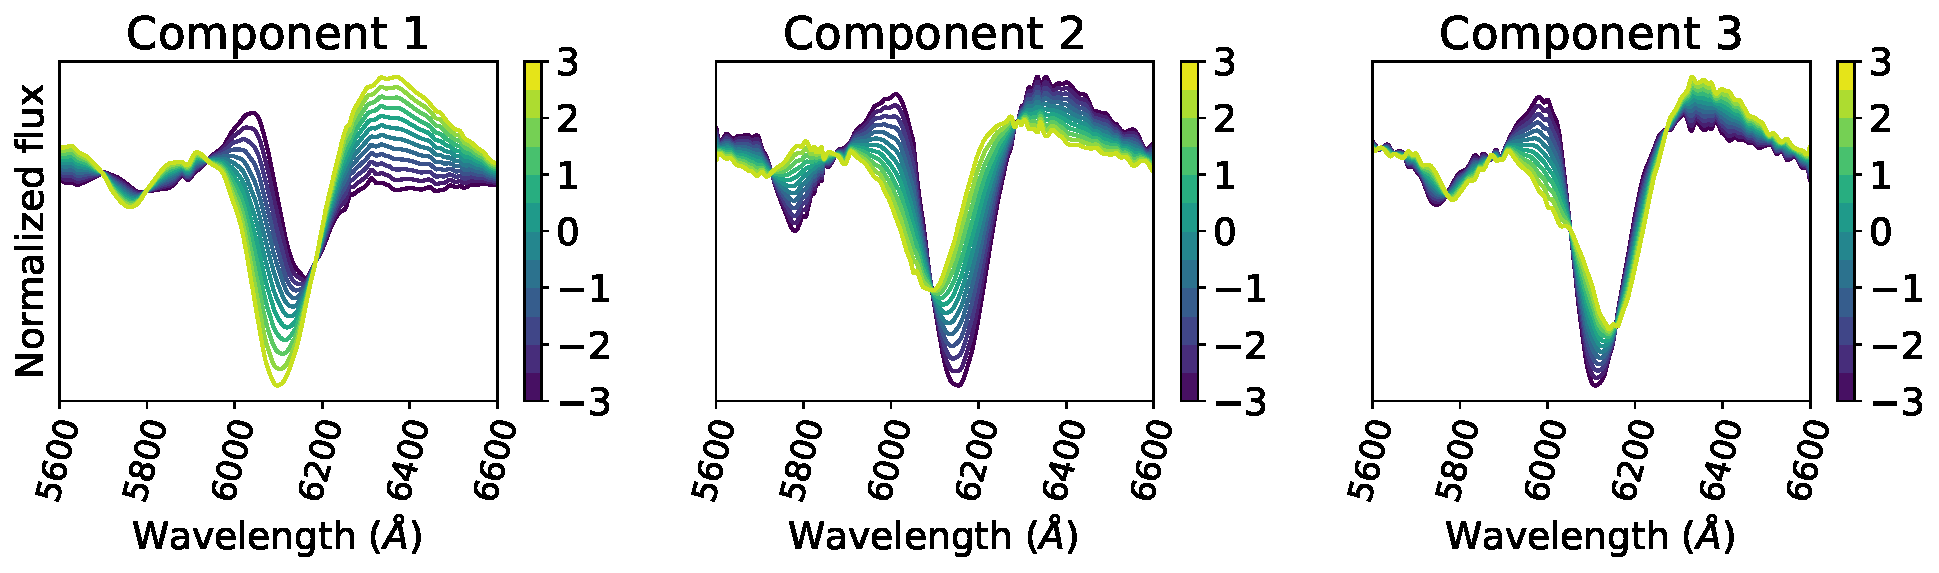
\includegraphics[width=0.9\textwidth]{figures/si_feat_pca/model_components.pdf}
    \caption{Visualization of the components ($\bm{x}$) of the EMFA model. Each subfigure shows the effect of adding various values of multiples of the components to the mean vector.}
    \label{emfa_components}
\end{figure}

The distributions of the loading coefficients are shown in Figure \ref{corner_plot_vel} and \ref{corner_plot_ew}. The qualitative observations about the relationship between the loading coefficients and the velocity and equivalent widths of the feature are confirmed there, as well as in Figure \ref{scatter_loading} where the spectral indicator measurements are plotted directly against the loading coefficients of each object in the training sample.

\begin{figure}[htbp]
    \centering
    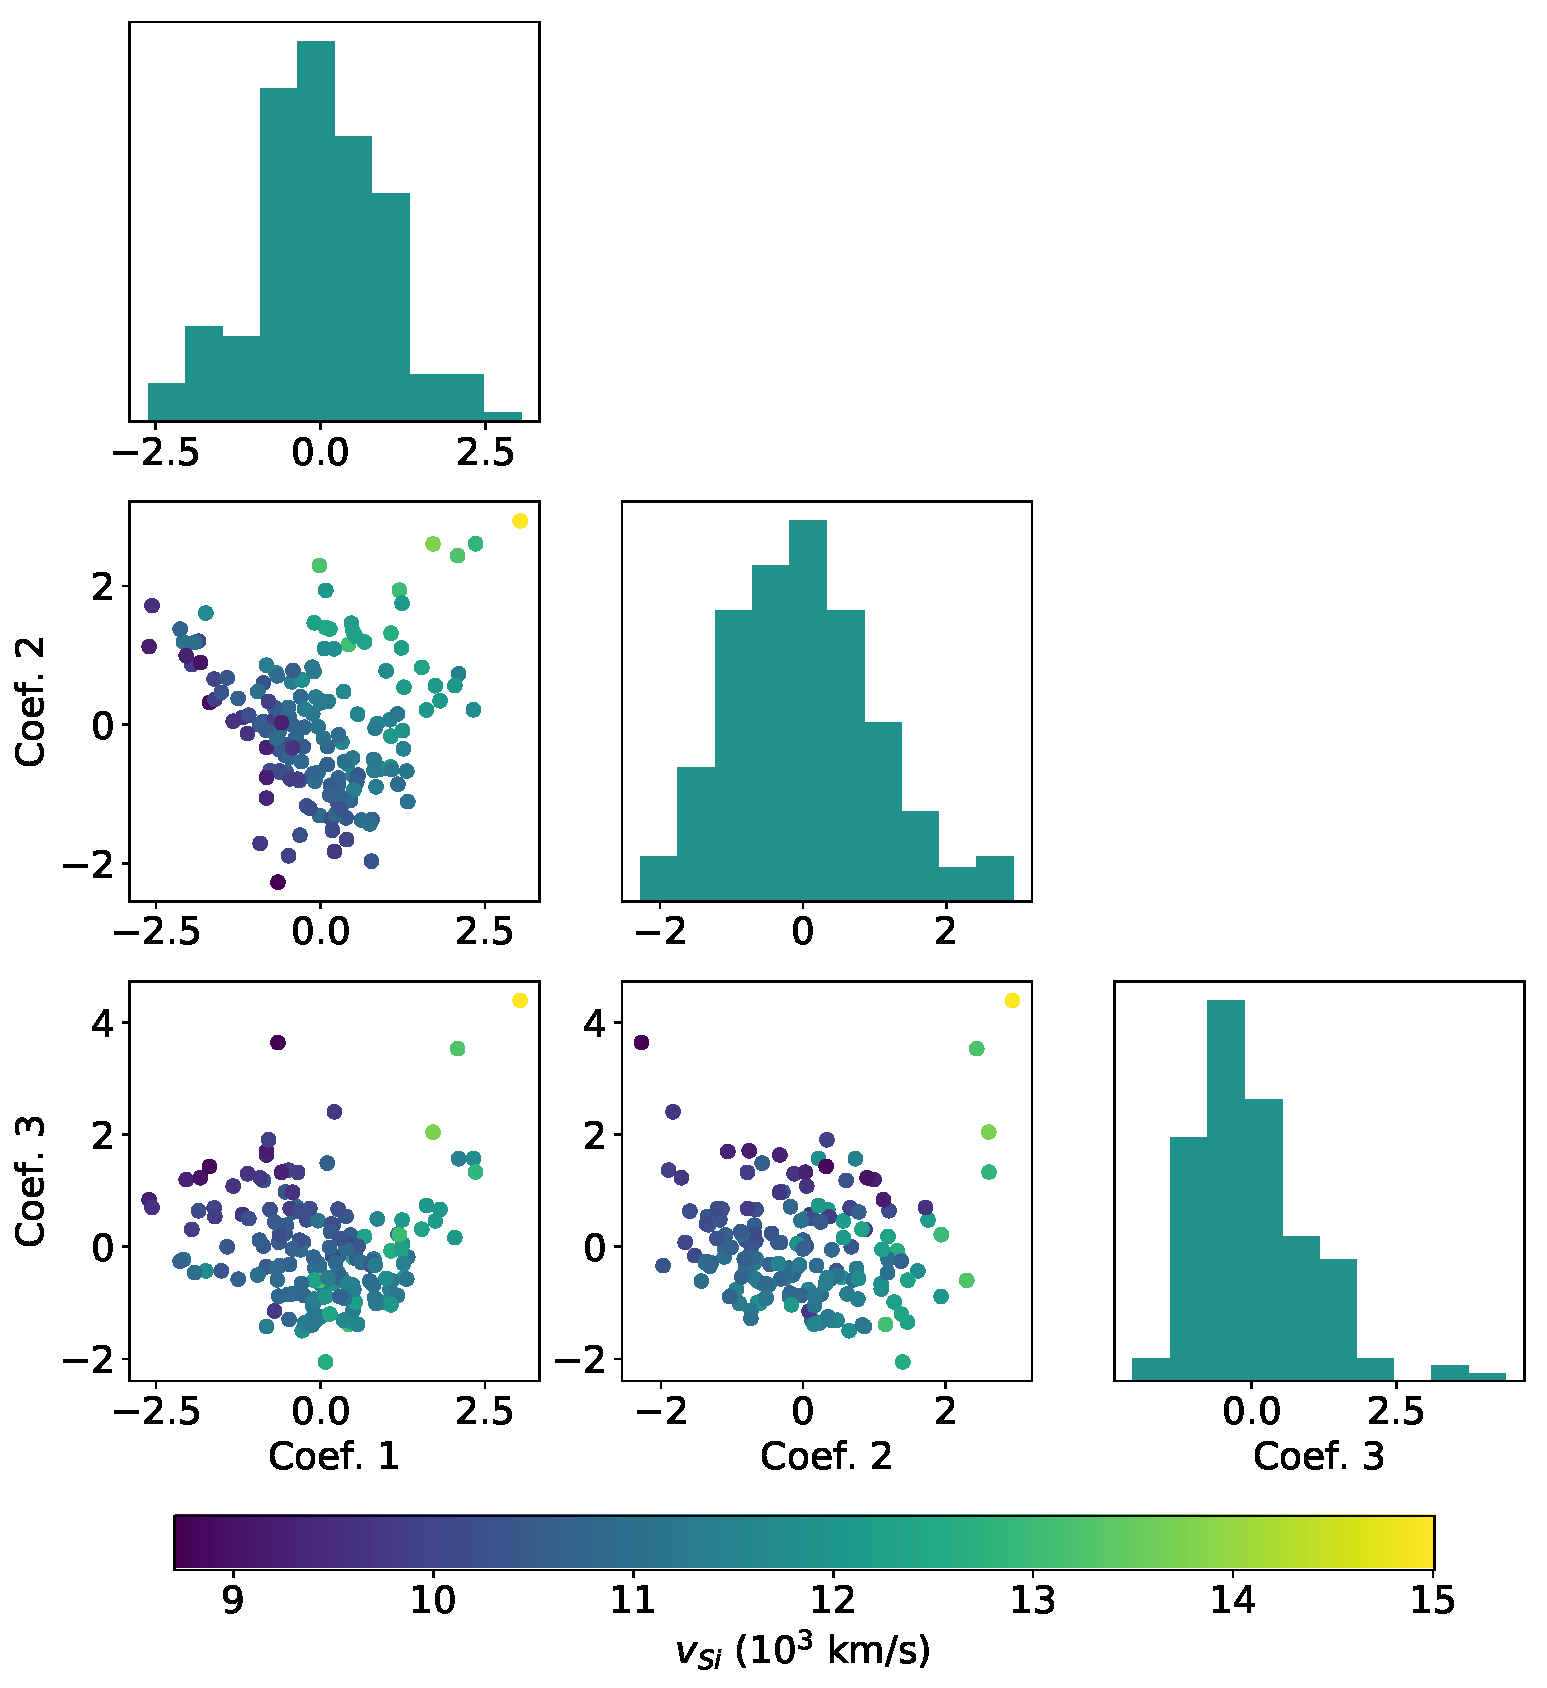
\includegraphics[width=0.9\textwidth]{figures/si_feat_pca/corner_plot_vel.pdf}
    \caption{Corner plot showing the marginal distributions of the loading coefficients for the training set, colored by the measured velocity of the \siliconii{} feature. Each point in the scatter plot represents one supernova.}
    \label{corner_plot_vel}
\end{figure}

\begin{figure}[htbp]
    \centering
    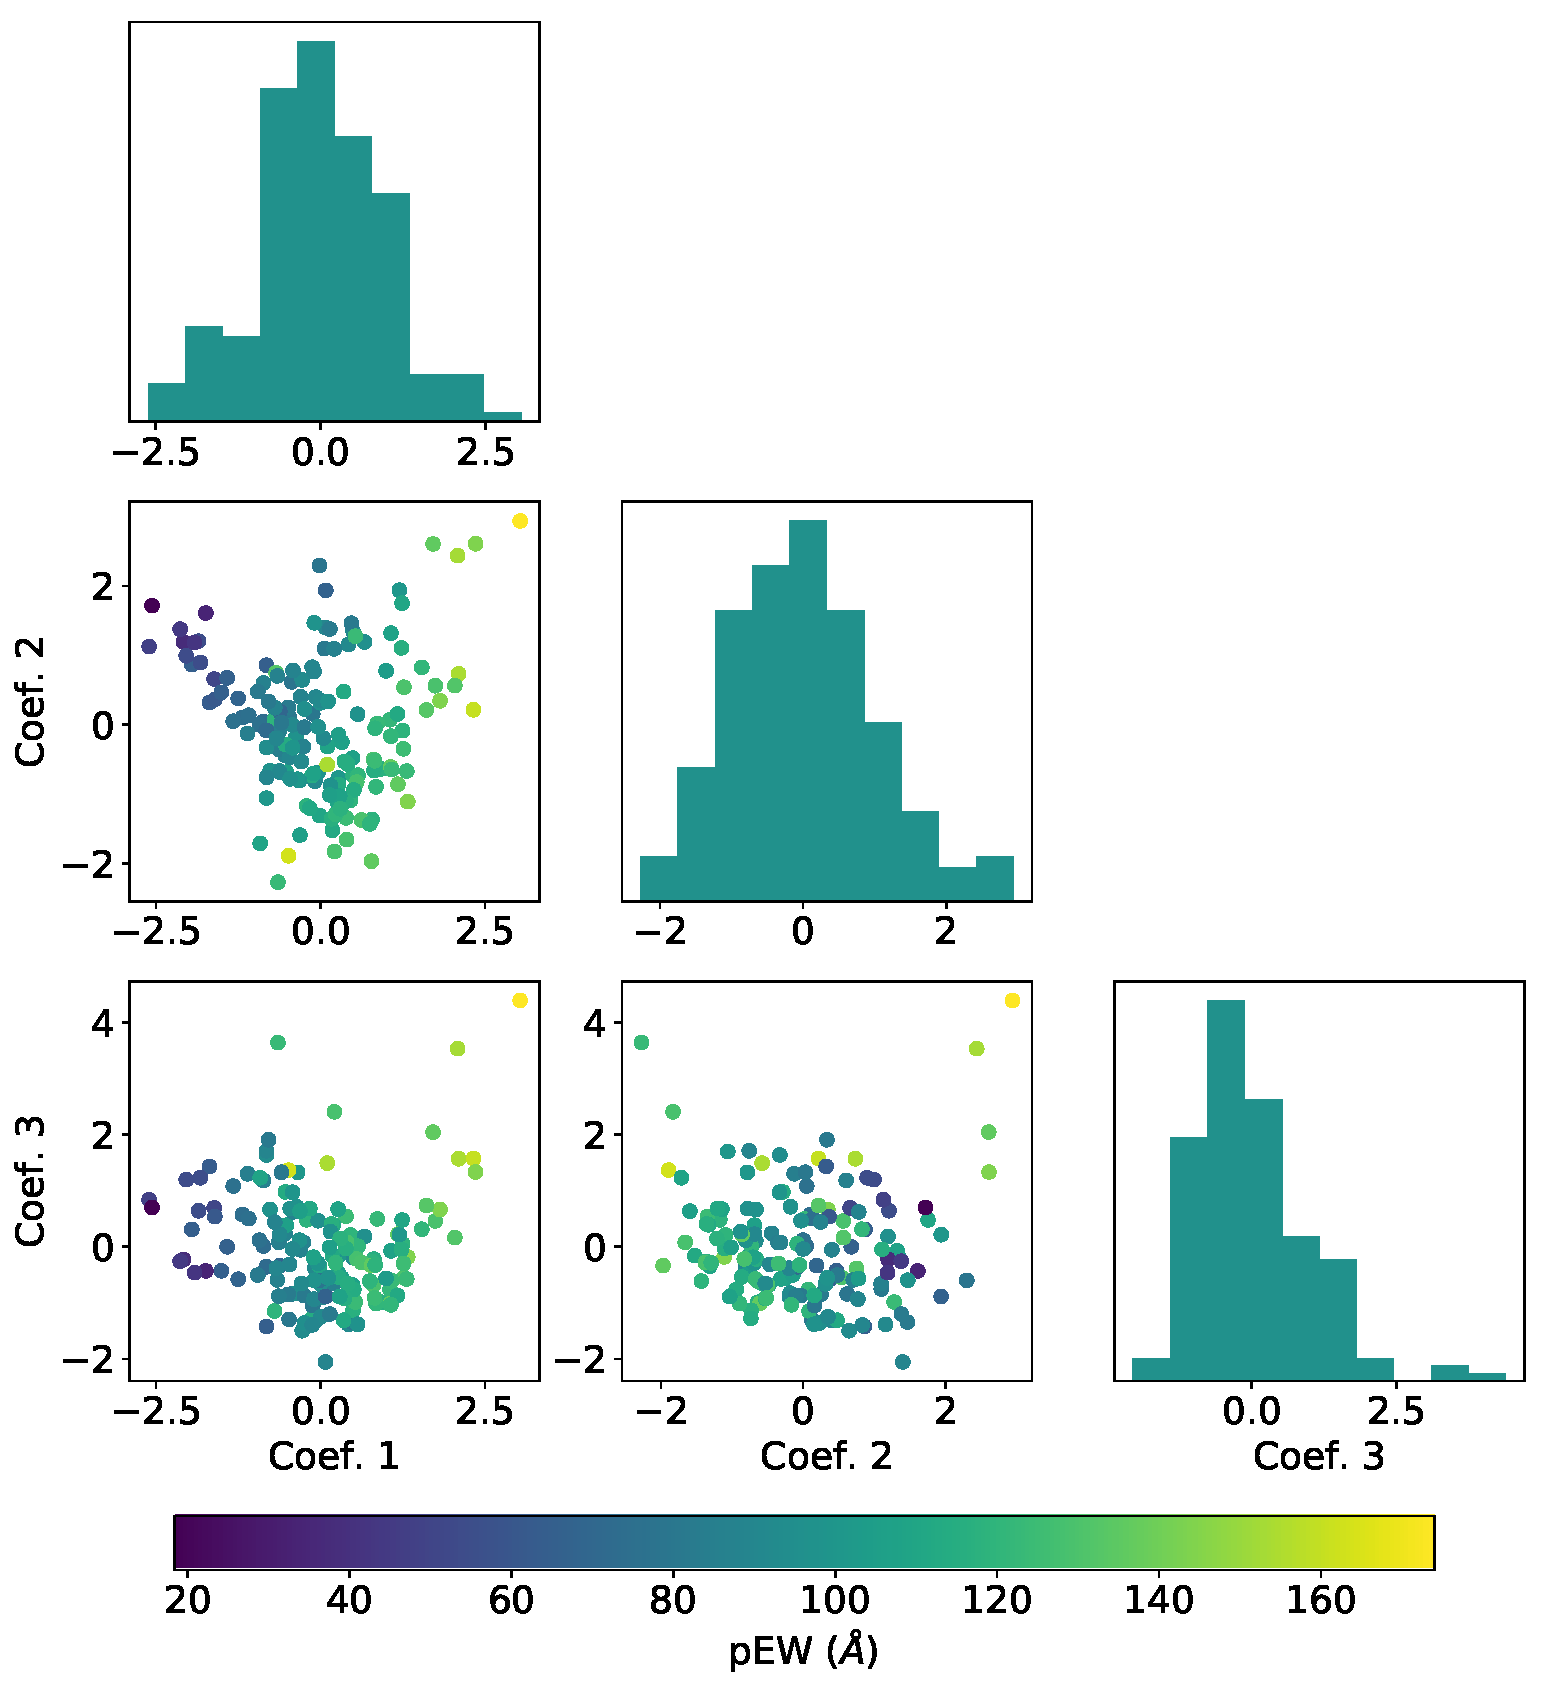
\includegraphics[width=0.9\textwidth]{figures/si_feat_pca/corner_plot_ew.pdf}
    \caption{Same as Figure \ref{corner_plot_vel}, but colored by the pseudo-equivalent width.}
    \label{corner_plot_ew}
\end{figure}

\begin{figure}[htbp]
    \centering
    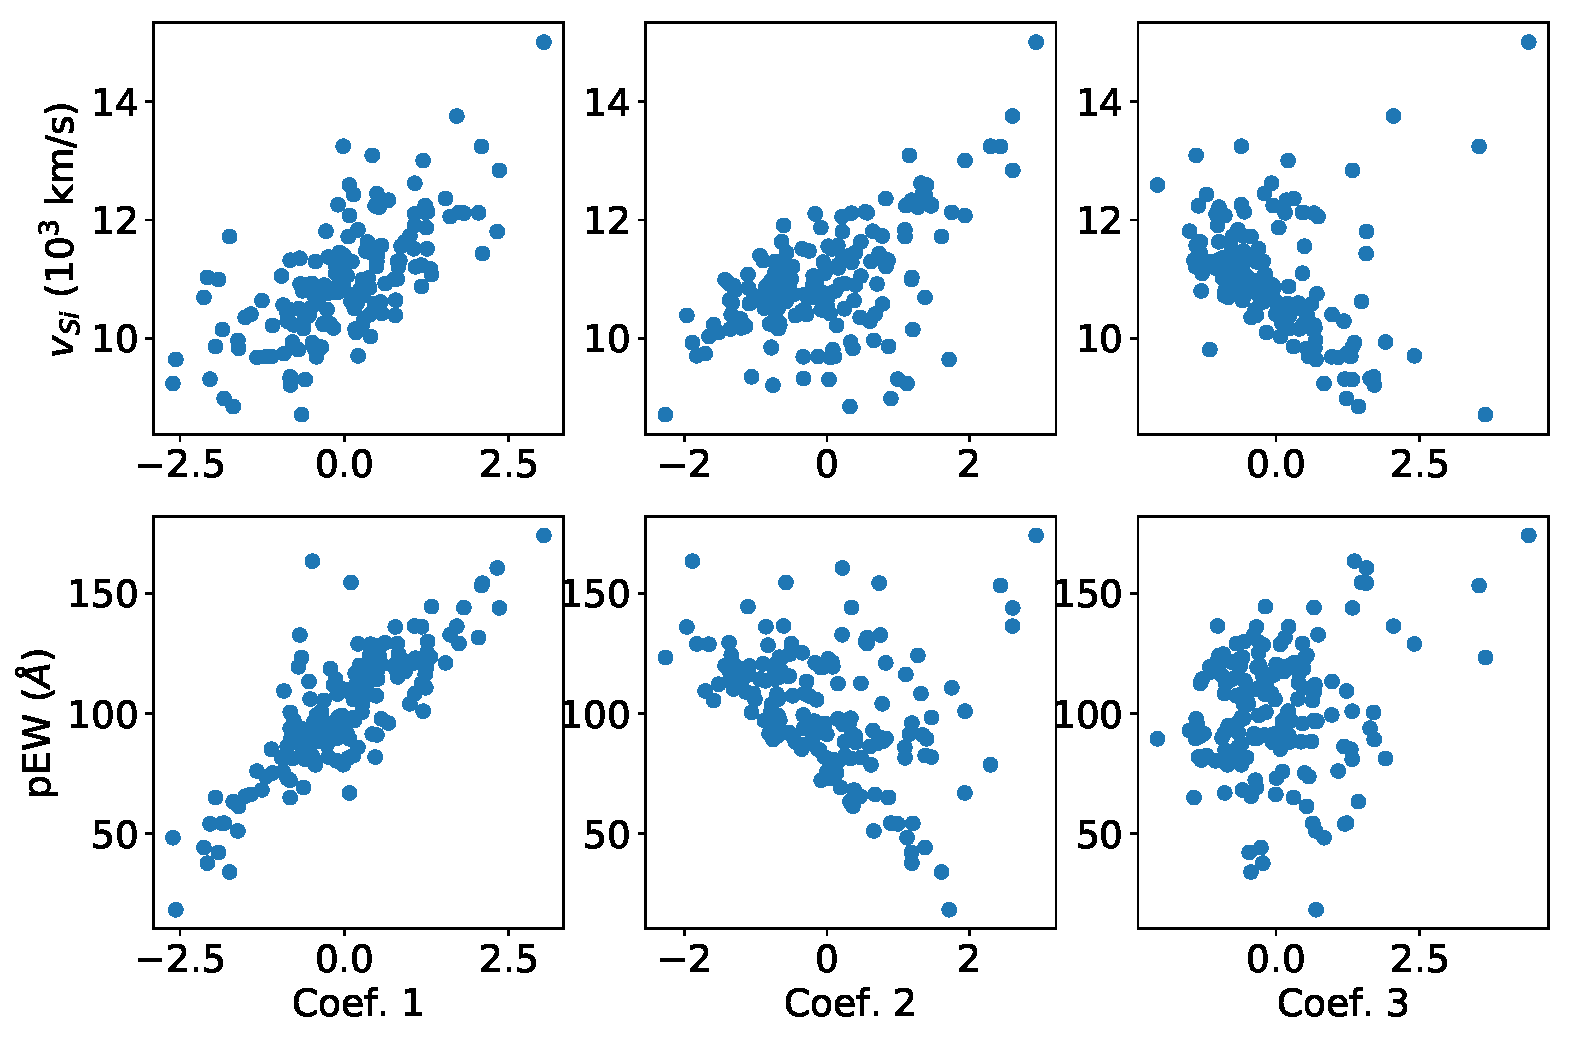
\includegraphics[width=0.9\textwidth]{figures/si_feat_pca/coef_vs_vel_and_ew.pdf}
    \caption{Scatter plots of the loading coefficients of the training data with their measured spectral indicators. We can see that each of the components is correlated with the velocity. Only the first two components are correlated with the pseudo-equivalent width.}
    \label{scatter_loading}
\end{figure}

\section{Validation}
\label{validation}

\subsection{Recovering Spectral Features at Native Resolution}
\label{snf_validation}
We can recover the spectral indicator measurements by reconstructing the full spectral feature from the EMFA model and measuring the velocity and equivalent width of the resulting reconstruction. When reasonably high resolution spectra are available, this reconstruction is unnecessary, so the native resolution recovery presented here is meant to provide a baseline estimate of how well the EMFA model can capture the inherently non-linear \siliconii{} features. It's real power will come into play when we estimate the velocity and pseudo-equivalent width from lower resolution or noisier spectroscopy.

Some examples of the feature recovery at native resolution are shown in Figure \ref{feature_recovery}. The histogram of residuals is shown in Figure \ref{snf_hist_resids_native_resolution}. The width of these distributions tells us how well the EMFA is capturing the spectral features. We find that the standard deviations (equivalently the root-mean-square or RMS) of these residual distributions are 369~km/s and 5.8~\,\AA{}, respectively. The normalized median absolute deviations\footnote{$$NMAD=1.4826\times\textrm{med}(|\bm{x}-\textrm{med}(\bm{x}|)$$} of these distributions are 253~km/s and 3.6~\,\AA{}. These errors in the recovery values are comparable to the average error on the original measurements (385~km/s for velocity and 6.8~\,\AA{} for the pseudo-equivalent widths).

\begin{figure}[htbp]
    \centering
    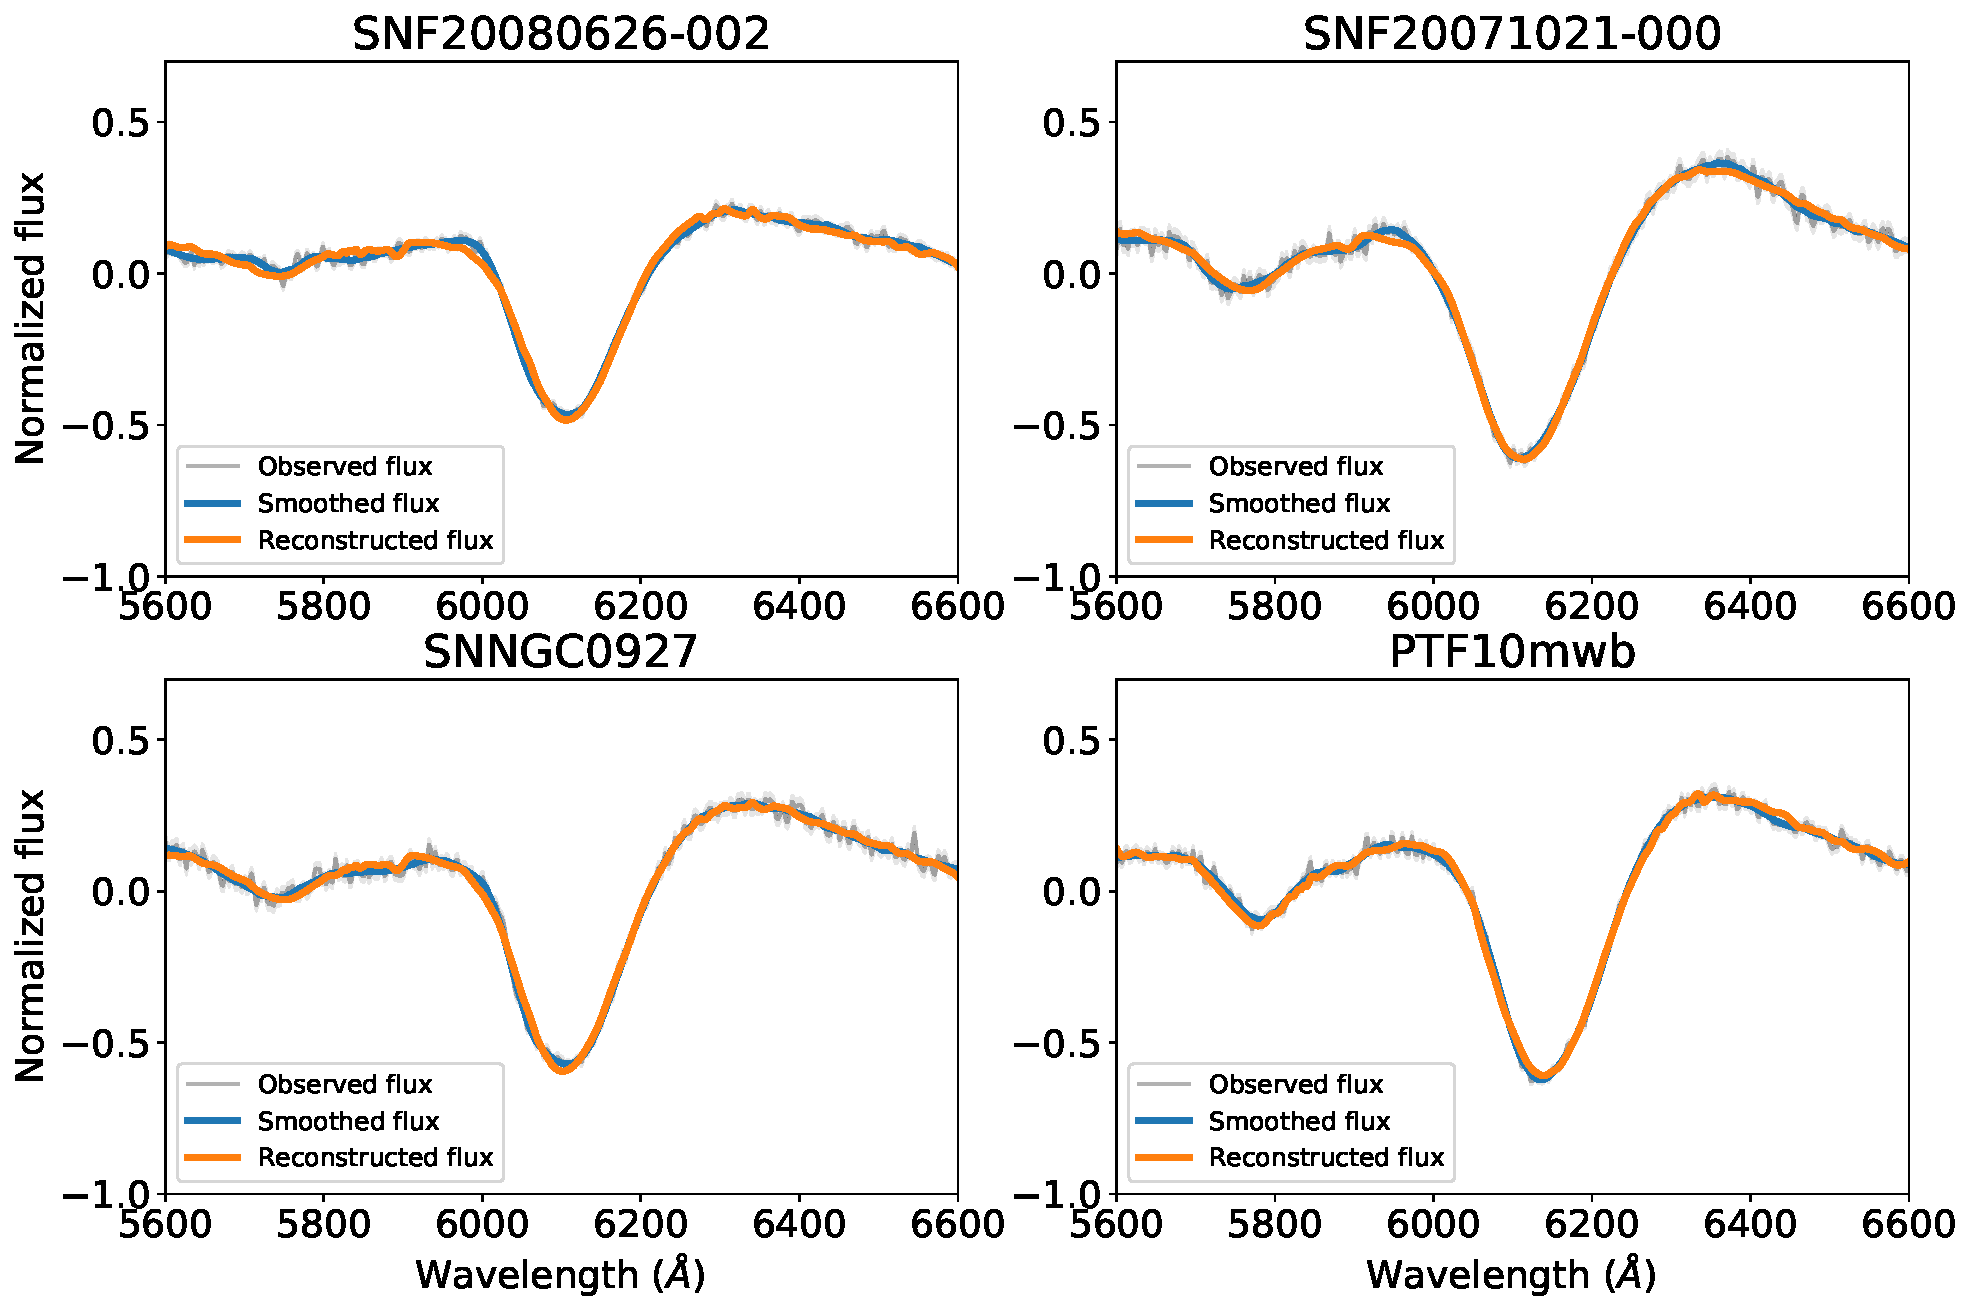
\includegraphics[width=0.9\textwidth]{figures/si_feat_pca/example_reconstruction.pdf}
    \caption{A random selection of recovered spectral features at the native resolution of the SNfactory spectra. The gray lines show the observed data, the blue line shows the data smoothed by the optimal Savitzky-Golay filter, and the orange line is the reconstructed flux.}
    \label{feature_recovery}
\end{figure}

\begin{figure}[htbp]
    \centering
    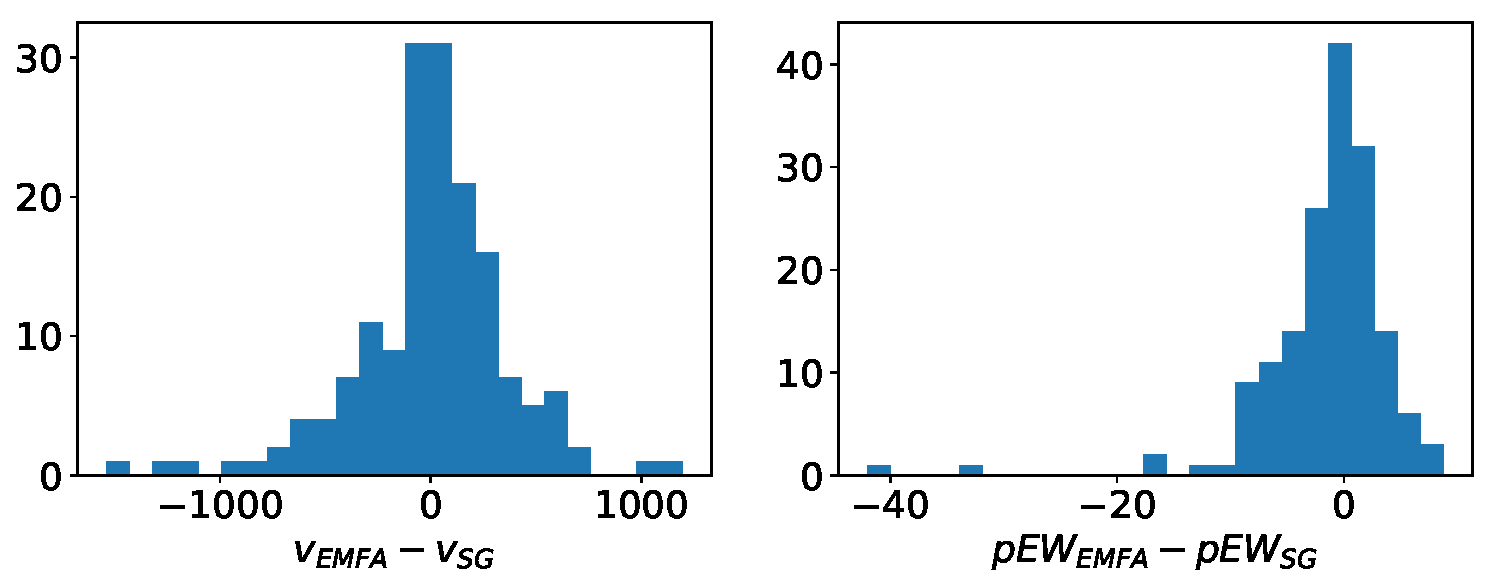
\includegraphics[width=0.9\textwidth]{figures/si_feat_pca/snf_recovery_resids.pdf}
    \caption{Histograms of the residuals between the velocities and equivalent widths measured from the flux reconstructed using the EMFA model and the original observed flux in the training data.}
    \label{snf_hist_resids_native_resolution}
\end{figure}

\section{Testing on External Data}
In order to ensure that our model is not overfit to our training data, we evaluate the effectiveness of our EMFA of the \siliconii{} feature on our external data set from the Berkeley SuperNova Ia Project \citep[BSNIP,][]{silverman_berkeley_2012} described in Section \ref{data}. Using the same techniques as in Section \ref{snf_validation}, we compare the velocities and pseudo-equivalent widths of the features inferred from the EMFA model and the true measured spectral indicators from the BSNIP spectra rebinned into a similar spectral resolution as the SNfactory training spectra. Figure \ref{bsnip_hist_resids} shows the residuals between the spectral indicators measured from the EMFA fits and the originally measured values. The results for both the SNfactory validation and the BSNIP test are all summarized in Table \ref{validation_results}. The spreads of these distributions are slightly larger than those of the training sample, and we investigate some causes for this in Section \ref{outliers}.

\begin{figure}[htbp]
    \centering
    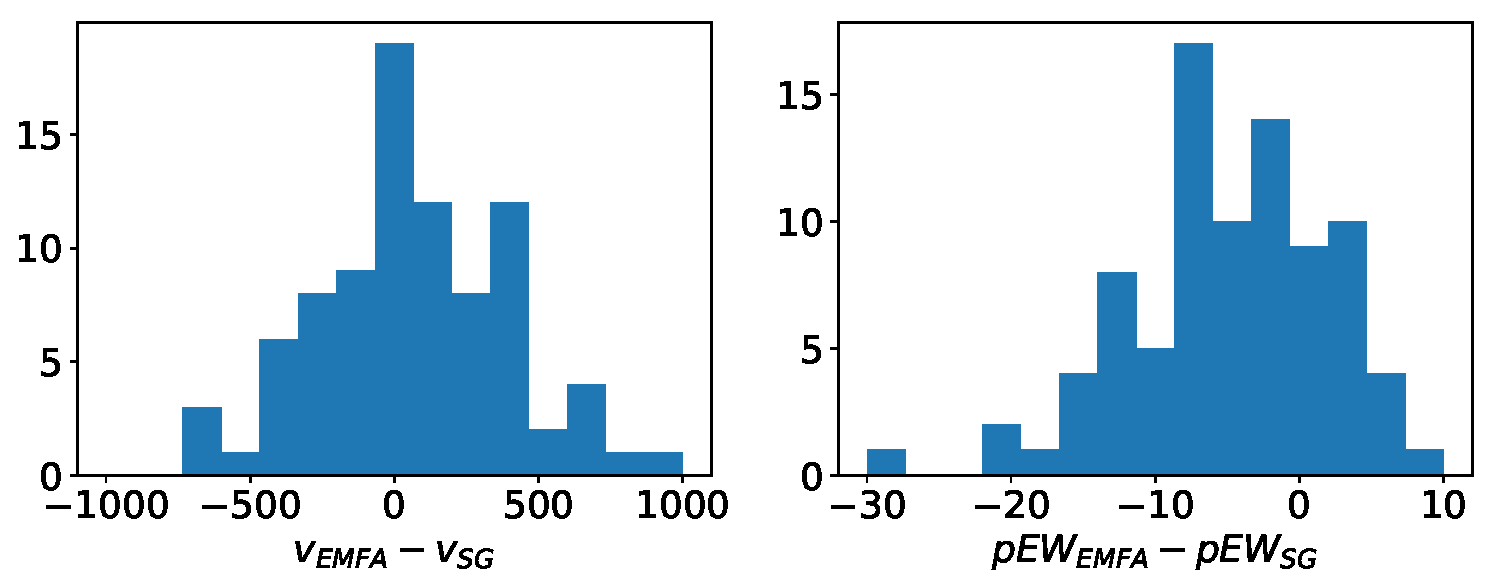
\includegraphics[width=0.9\textwidth]{figures/si_feat_pca/bsnip_recovery_resids.pdf}
    \caption{Histograms of the residuals between the velocities and equivalent widths measured from the flux reconstructed using the EMFA model and the original observed flux in the validation set. The outlier SN2005M has been removed from these plots (see Section \ref{outliers})}
    \label{bsnip_hist_resids}
\end{figure}

\begin{table}[htbp]
    \centering
    \begin{tabular}{ccccc}\\\toprule
        & \multicolumn{2}{c}{Velocity resids.} & \multicolumn{2}{c}{Equiv. width resids.}\\
        & \multicolumn{2}{c}{(km/s)} & \multicolumn{2}{c}{(\,\AA)}\\
        Data set & RMS & NMAD & RMS & NMAD\\\midrule
        SNfactory & 369 & 253 & 5.8 & 3.6 \\
        BSNIP & 392 & 355 & 7.7 & 7.1 \\\bottomrule
    \end{tabular}
    \caption{Measurements of the spread of the residuals between spectral features measured from the EMFA modeled spectra and spectral features measured from the true spectra for both the SNfactory (training) set and the BSNIP (test) set.}
    \label{validation_results}
\end{table}

\subsection{Investigating Large Residuals}
\label{outliers}
There are a few failed reconstructions from our validation. We show them in Figure \ref{valid_failures}, and discuss them here.

\begin{figure}[htbp]
    \centering
    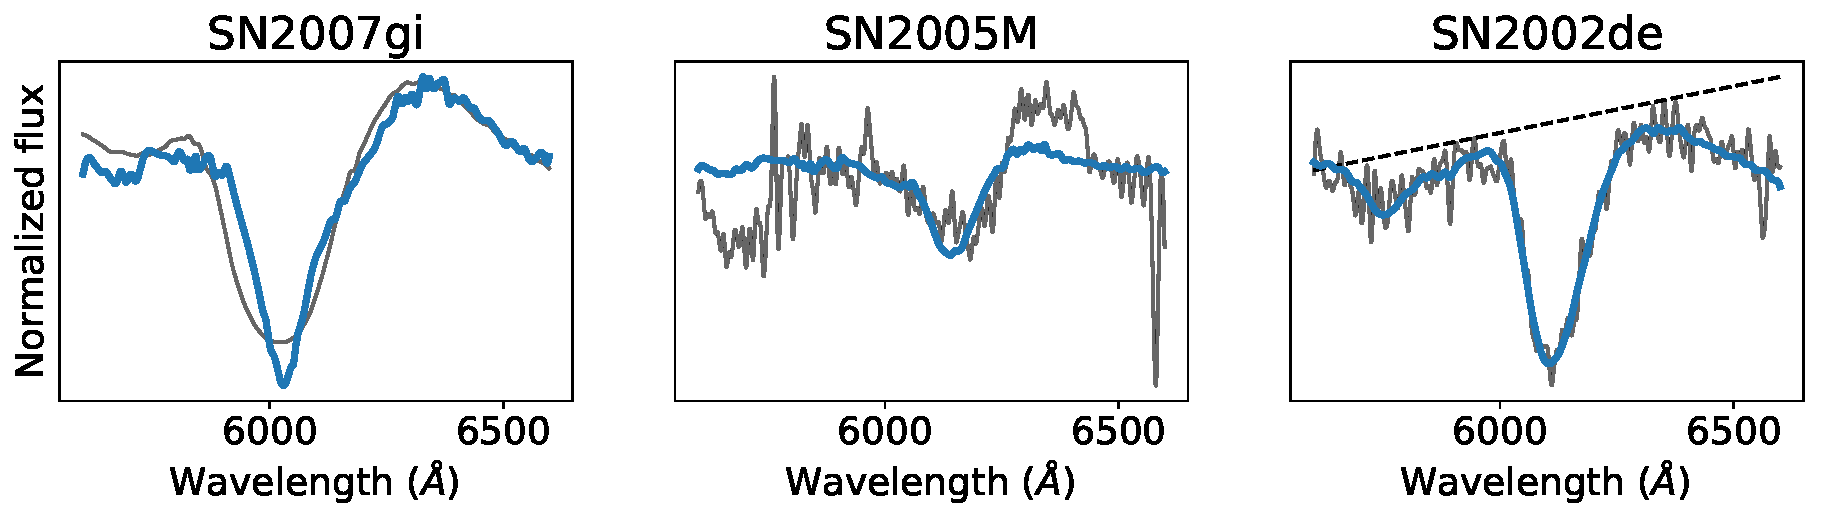
\includegraphics[width=\textwidth]{figures/si_feat_pca/fit_failures.pdf}
    \caption{Validation spectra where the EMFA fit and/or pseudo-continuum determination failed. The left frame is SN2007 gi, an exremely rapidly expanding object. The middle frame is SN2005M, which may be 1991T-like. The right frame shows an example of an object for which the pseudo-continuum determination failed due to underestimated variance in the spectrum. In each subfigure, the gray line represents the SG smoothed flux, and the blue line shows the best-fit EMFA flux. In the right figure, we also show the pseudo-continuum as a dashed black line.}
    \label{valid_failures}
\end{figure}

SN2007gi was a very well observed object with a high signal-to-noise spectrum, and thus precise measurements of the spectral indicators. Though the size of the residual was within the usual uncertainty of a measurement from a moderately well-observed spectra, the residual for this object was significantly larger than the measurement uncertainty. Looking at the recovered flux, we see that the EMFA model flux doesn't match the observed flux. SN2007gi is an extremely high velocity object ($v_{Si}=15740\pm180$~km/s with a large equivalent width ($pEW=176.9\pm1.6$~\,\AA{}), indicating that we may be somewhat limited by the diversity of our training set.

SN2005M was also a significant outlier. SN2005M has the shallow silicon lines of a SN1991T-like object, but a low velocity ($8300\pm 260$~km/s) that is uncharacteristic of SN1991T-like objects, which have typical velocities of $\sim 10000$~km/s \citep{blondin_spectroscopic_2012}. Since such shallow line objects were explicitly excluded from our training data set, the model is unable to capture this variation.

By eye checks of the remaining objects with large pseudo-equivalent width residuals reveal that it is not the EMFA that is failing to capture the feature, but failures in the pseudo-continuum determination in the SG filtering process. Usually, this is due to the variance spectra being underestimated, resulting in undersmoothing of the curve, and the limits of the pseudo-continuum being determined by noise spikes. An example of this is shown in the final panel of Figure \ref{valid_failures} for SN2002de. We conclude that, aside from the specific outliers of SN2007gi and SN2005M, the slightly larger spread in our validation residuals is driven by this variance underestimation in the validation data set, and not overtraining of our model.

\section{Simulated Roman Prism Spectra}
\label{wfirst}
\subsection{Generating Roman Prism Spectra}
The Nancy Grace Roman Space Telescope (hereafter Roman) is a future space telescope mission designed to constrain cosmological parameters with wide-field optical and near-infrared imaging. In addition to the imaging instrument (the Wide Field Channel, or WFC), a low-dispersion slitless prism has also been proposed as a tool to obtain spectroscopy for SNe Ia.

The full details of the prism simulation we use in this section can be found in Rubin et al. (in preperation), but we will present a summary here. The prism is still in design stages, so we assume a similar dispersion to the previously proposed Integral Field Channel (IFC), but with narrower wavelength coverage (0.7 to 1.8 $\mu$m). The survey simulation assumes an exposure time of one hour per pointing. This yields the at-max signal-to-noise ratios shown in Figure \ref{snr_wfirst_prism}, where we report the average signal-to-noise ratio per pixel from 5600-6600~\,\AA{} in the rest frame (the wavelength region of interest for this chapter). The average signal-to-noise ratio is calculated for a normal SN Ia in 38 evenly spaced redshift bins from 0.125 to 1.175. It is worth noting that the parameters of this survey (the wavelength coverage, dispersion, exposure times, etc) have not been optimized in any way; this survey serves as a benchmark for the spectral indicator measurement technique discussed here. Future work can use these analyses to find a more optimal survey strategy and instrument design.

\begin{figure}[htbp]
    \centering
    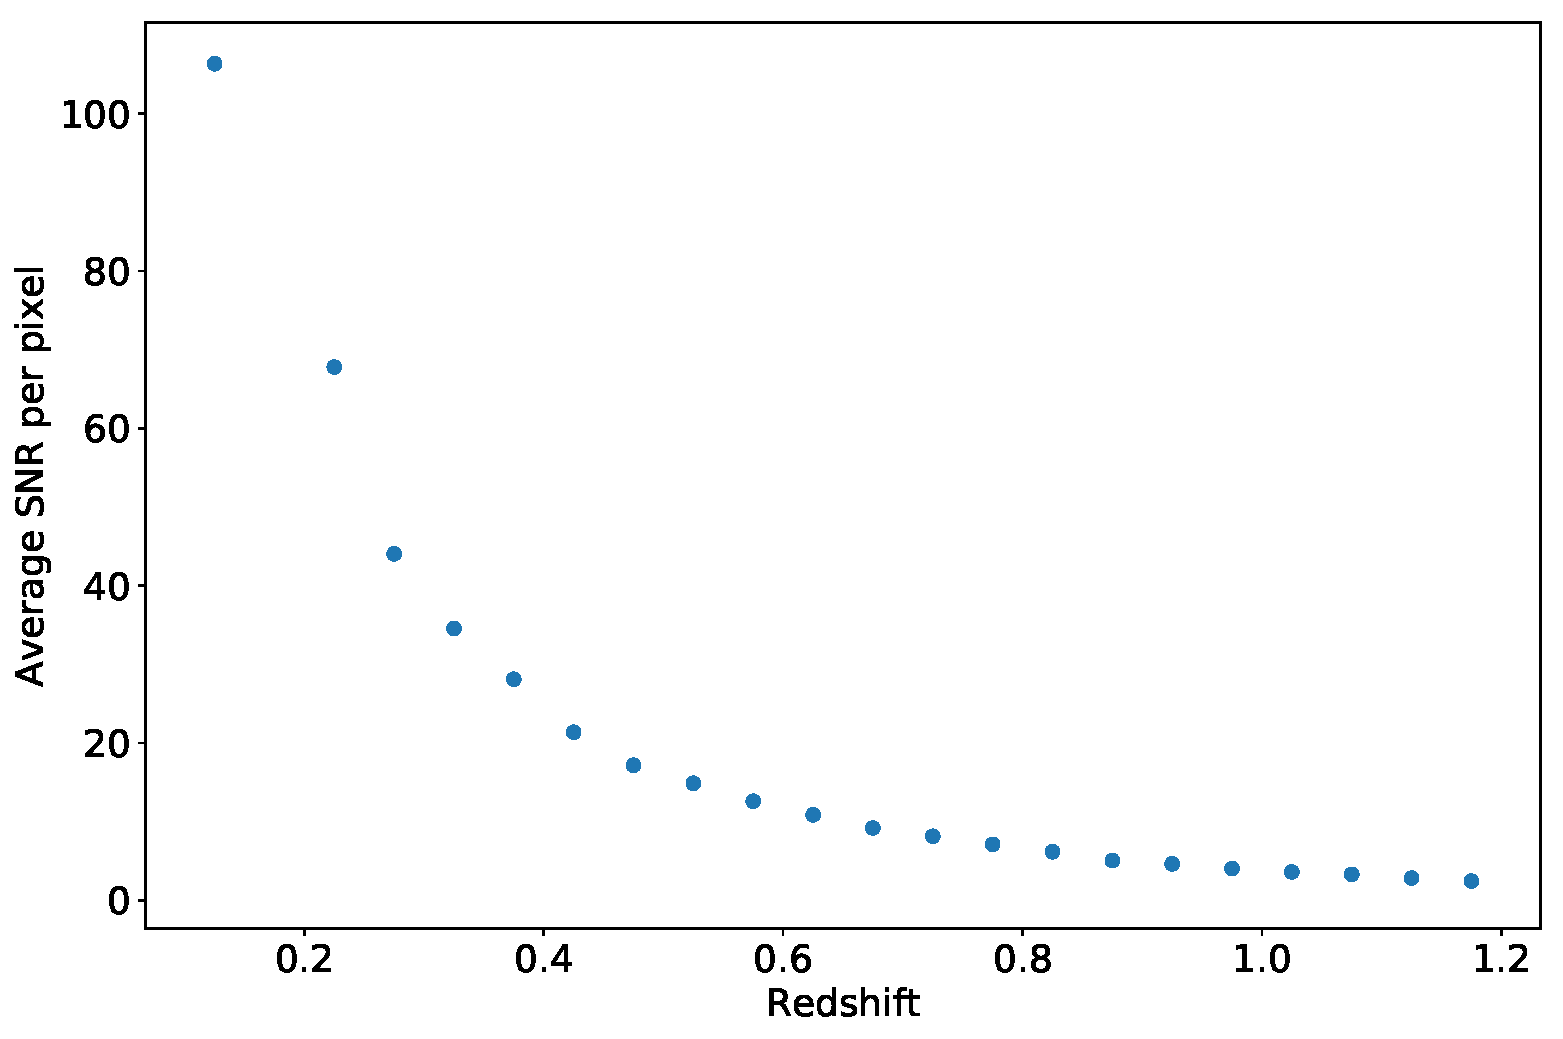
\includegraphics[width=0.9\textwidth]{figures/si_feat_pca/wfirst_snr_vs_redshift.pdf}
    \caption{Average signal-to-noise ratio for assumed for prism spectra used in the simulations. We report the average from 5600-6600~\,\AA{} in the rest frame since this is the wavelength region of interest.}
    \label{snr_wfirst_prism}
\end{figure}

The simulated data set is generated as follows. For each object in the training set and for each redshift bin, we artificially redshift the spectrum to the redshift of the bin, resample the spectrum into the resolution of the prism spectrograph, and generate 50 realizations of the noise. The separate realizations allow us to inspect how the uncertainty (our confidence in the measurement value due to noise fluctuations) changes with redshift (or S/N) for spectra at these resolutions as well as how the errors (systematic offsets between the model and the true underlying data) change with redshift. A few example Roman prism spectra in a range of redshifts are shown in Figure \ref{wfirst_example_spectra}.

\begin{figure}[htbp]
    \centering
    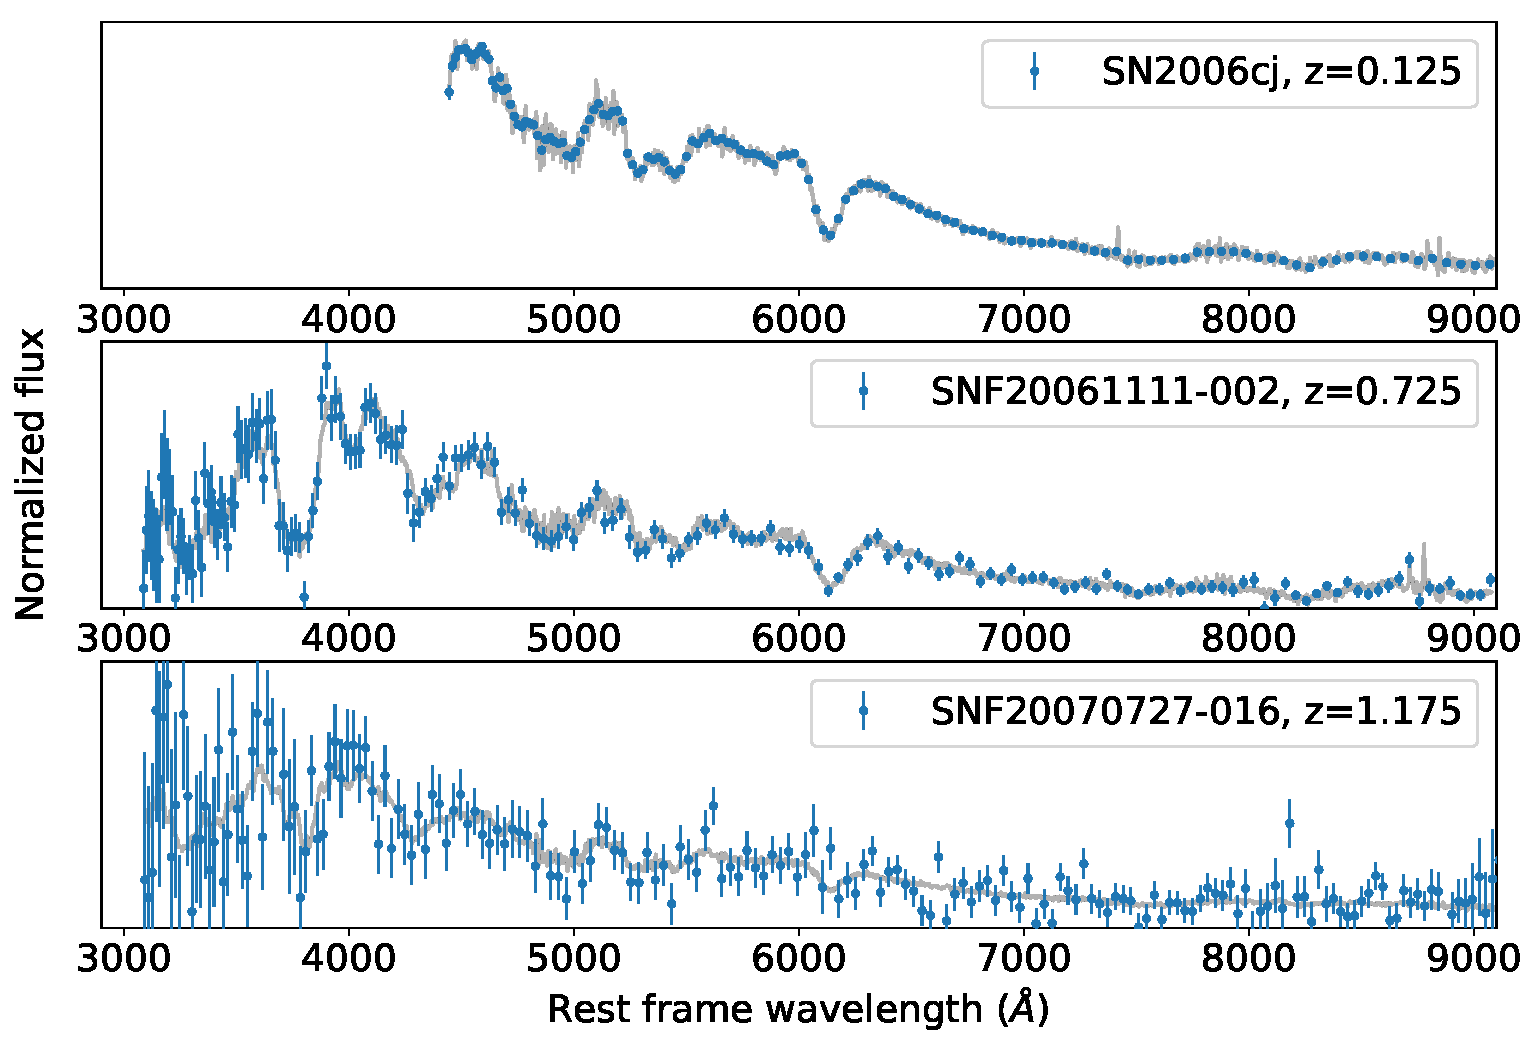
\includegraphics[width=0.9\textwidth]{figures/si_feat_pca/wfirst_example_spectra.pdf}
    \caption{Example realizations of the training set near-max spectra observed with the Roman prism spectrograph with a one hour exposure time.}
    \label{wfirst_example_spectra}
\end{figure}

Each of these spectra was preprocessed as described in Section \ref{data} and is available as part of the data repository accompanying this work.

\subsection{Spectral Indicator Recovery Results}
For every spectrum generated, we measured the velocity and pseudo-equivalent width using the SG smoothing, the Gaussian fit, and the EMFA fit methods. We then compared the results of these fitting methods to the true values of these spectral indicators (i.e. those measured from the original, high resolution, low noise spectra from the training sample).

In the validation step, the spectra we were fitting were at the same resolution as the training data. Therefore the data vectors had the same length and correspond to the same wavelengths as the training data, so we do not need to interpolate either the data or the model. Now we no longer have the same resolution, so we instead interpolate the model components using a spline and fit this interpolated model by minimizing
\begin{equation}
    \chi^2 = \displaystyle\sum_\lambda \frac{(f_{mod}(\lambda)-f_{obs}(\lambda))^2}{\sigma_{obs}^2(\lambda)}
\end{equation}
where $\lambda$ indexes the wavelength bins of the observation, $f_{mod}$ is the spline interpolated model spectrum evaluated at the wavelength bin $\lambda$, and $f_{obs}$ is the observed flux. An example of the recovered flux from one realization of one object is shown in Figure \ref{example_wfirst_recovery}.

\begin{figure}[htbp]
    \centering
    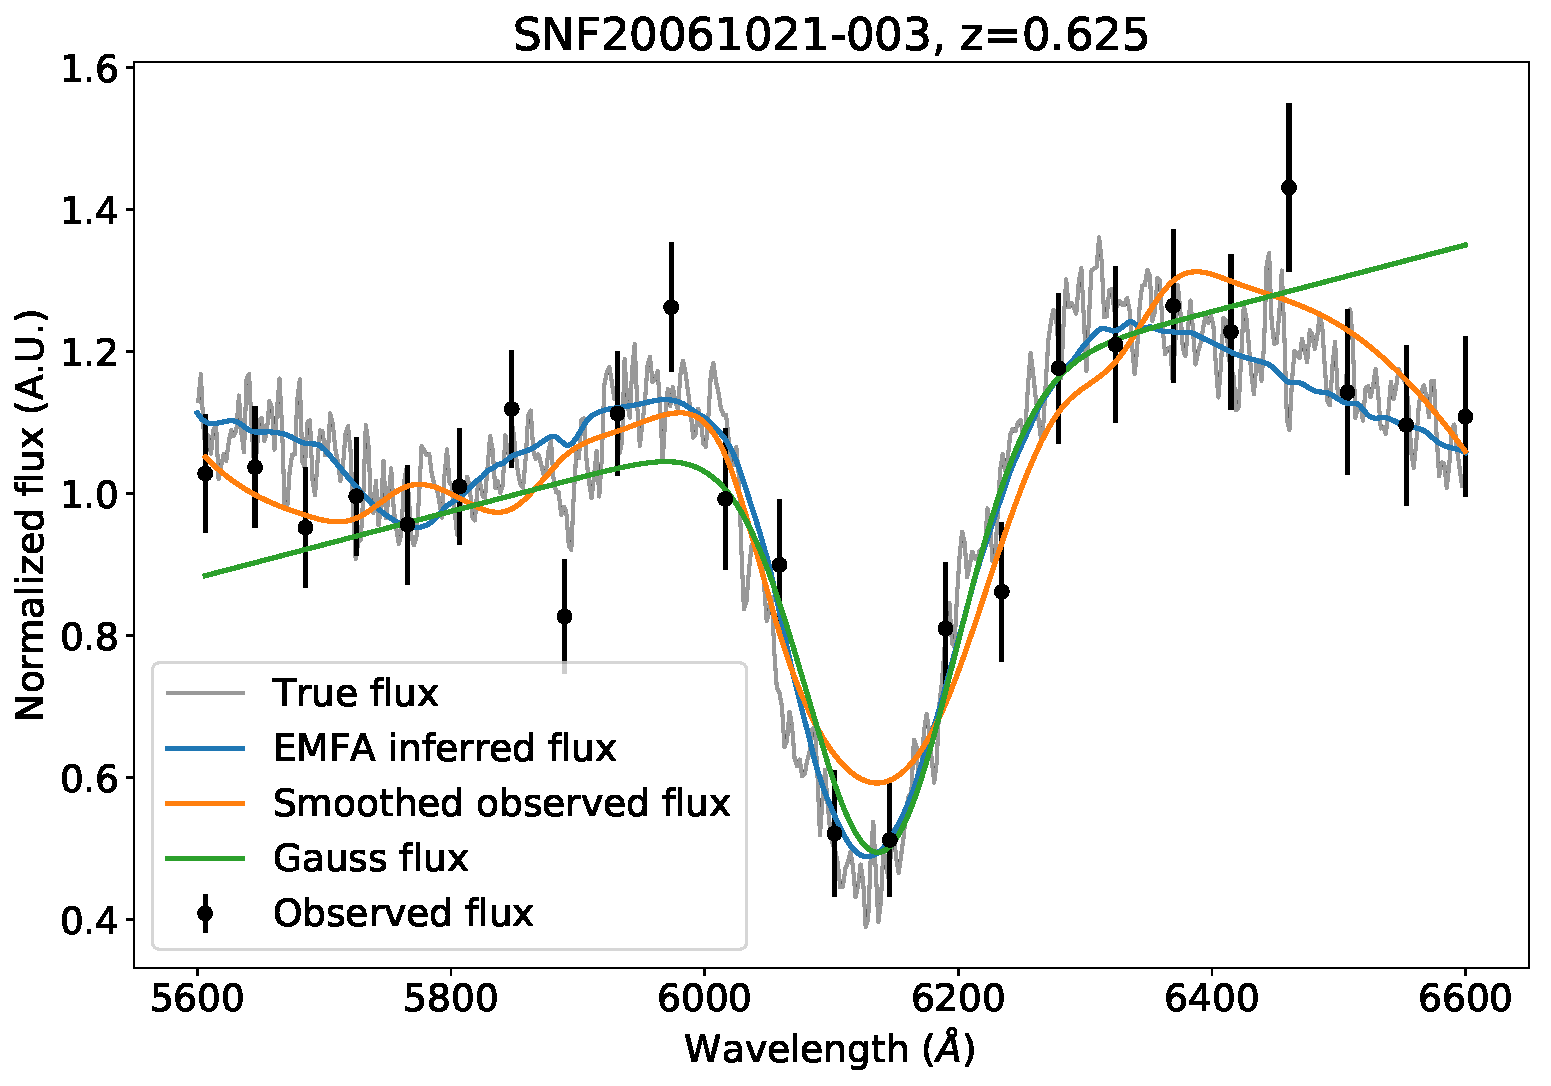
\includegraphics[width=0.9\textwidth]{figures/si_feat_pca/example_wfirst_emfa_recovery.pdf}
    \caption{Example of the various methods tested to recover the spectral indicators from the low resolution, noisy spectra from the Roman prism. The original training set spectrum that was resampled and noised is shown in gray. The realization of the prism observation (with uncertainties) is shown as the black data points. The best-fit EMFA spectral feature is shown in blue, the smoothed version of the observed flux is shown in orange, and the best-fit Gaussian line profile is shown in green.}
    \label{example_wfirst_recovery}
\end{figure}

First, we examine how the error in the measurements changes with redshift, where the error is defined by the difference between the measurements obtained from the noisy, degraded spectrum and the original data. Figure \ref{wfirst_vel_err_vs_z} and \ref{wfirst_ew_err_vs_z} show the average absolute difference between the velocities and pseudo-equivalent widths measured from the noisy data and those measured from the original data. At low redshifts (high signal-to-noise), each of the methods are roughly comparable. As the noise increases, though, the EMFA reconstruction does significantly better at recovering both the velocities and equivalent widths. Using the EMFA, we can obtain an estimate of the velocity to within 500 km/s out to a redshift of $z\sim0.75$, compared to $z<0.6$ with the SG filtering method. 

\begin{figure}[htbp]
    \centering
    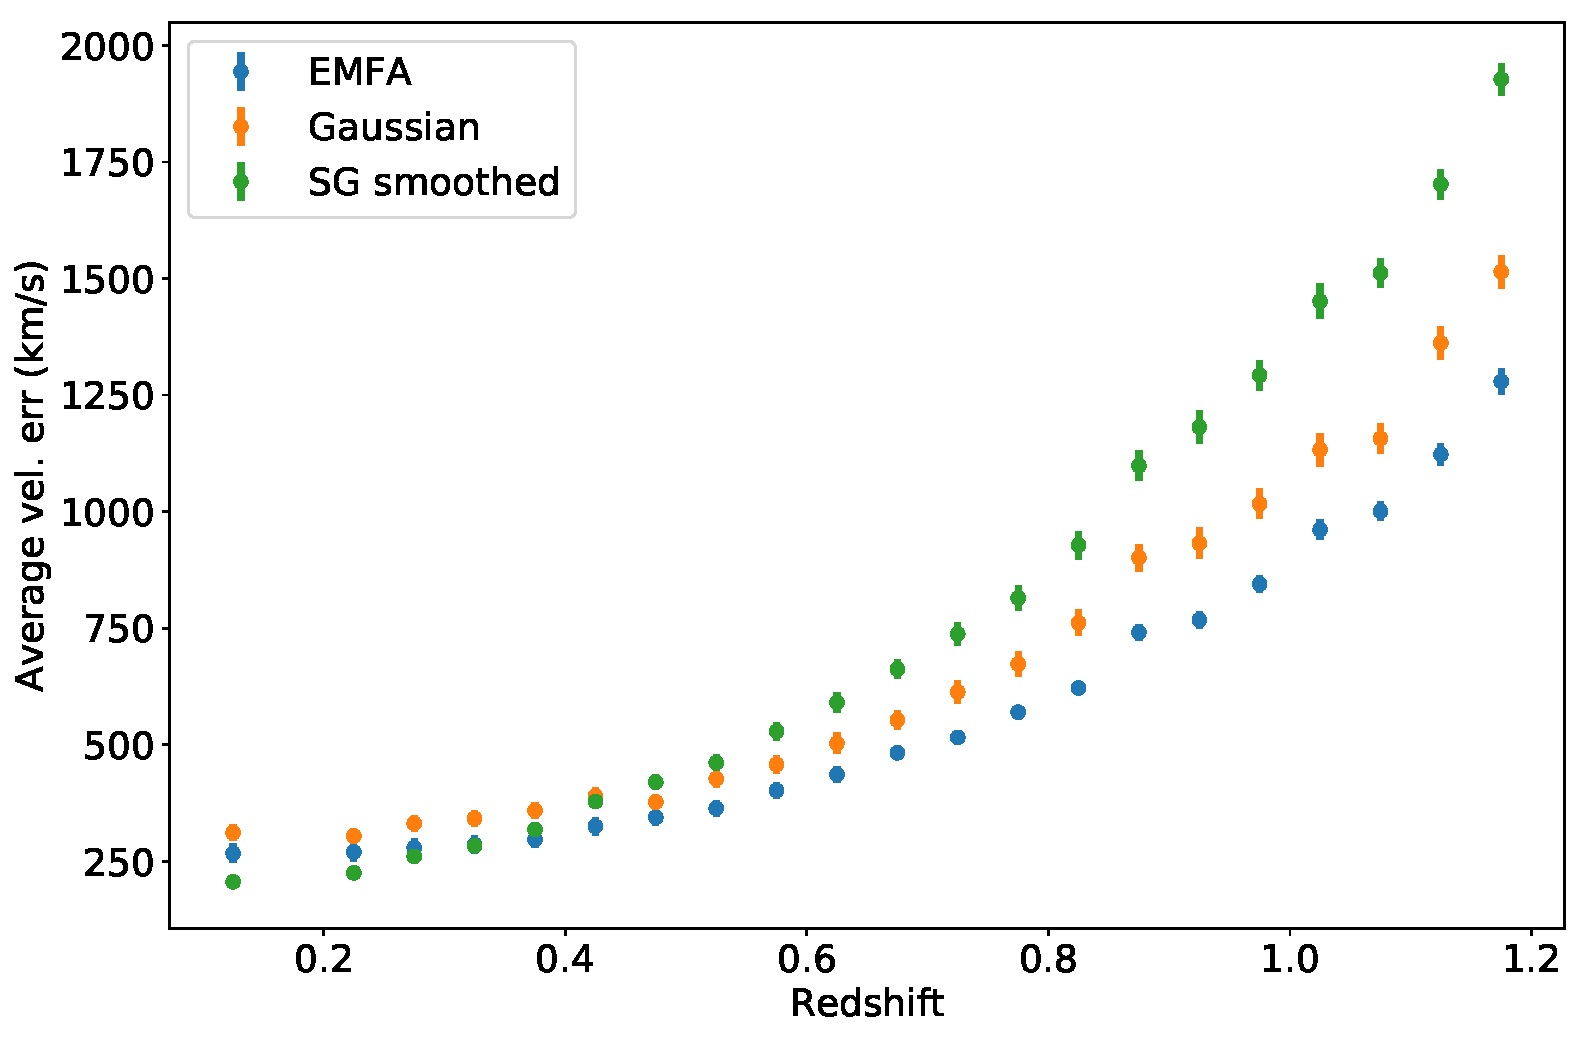
\includegraphics[width=0.9\textwidth]{figures/si_feat_pca/wfirst_vel_err.pdf}
    \caption{Per-redshift-bin average of the absolute value of differences between measured velocities and true velocities as a function of redshift for the simulated Roman prism spectra. At low redshifts, the SG filtering method captures the true value best, but as noise increases, the EMFA method outperforms all other methods.}
    \label{wfirst_vel_err_vs_z}
\end{figure}

\begin{figure}[htbp]
    \centering
    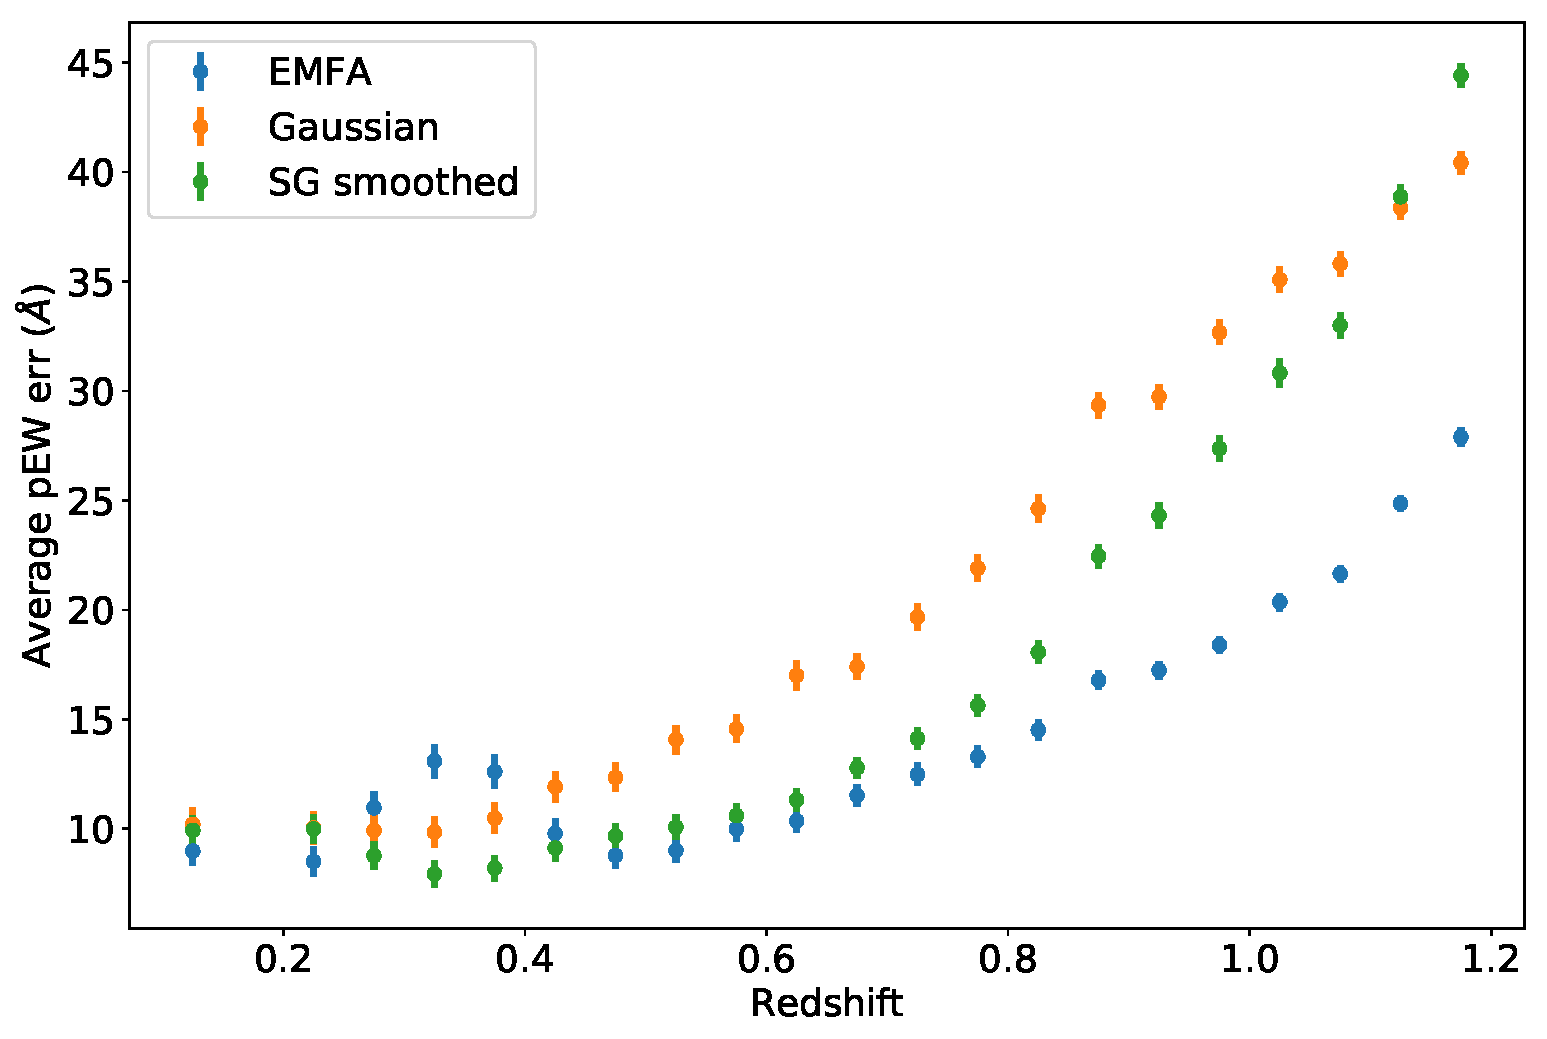
\includegraphics[width=0.9\textwidth]{figures/si_feat_pca/wfirst_pew_err.pdf}
    \caption{Same as Figure \ref{wfirst_vel_err_vs_z}, but for pseudo-equivalent width measurements. At low redshifts, all methods give comparable errors, but as the noise increases, the EMFA method is the preferred technique.}
    \label{wfirst_ew_err_vs_z}
\end{figure}

We also examine how the uncertainty in each of these measurements changes with the redshift in this prism survey. We look at the spread of the spectral indicator measurements among the 50 realizations of each object in each redshift bin. Figure \ref{wfirst_vel_uncertainty_vs_z} shows the average uncertainty of the velocity measurements as a function of redshift for each measurement technique. Figure \ref{wfirst_ew_uncertainty_vs_z} shows the same but for the pseudo-equivalent width measurements. Once again, we see that all measurement techniques are roughly comparable in both metrics at low redshift (high signal-to-noise). At higher redshifts, the EMFA again outperforms the other techniques.

\begin{figure}[htbp]
    \centering
    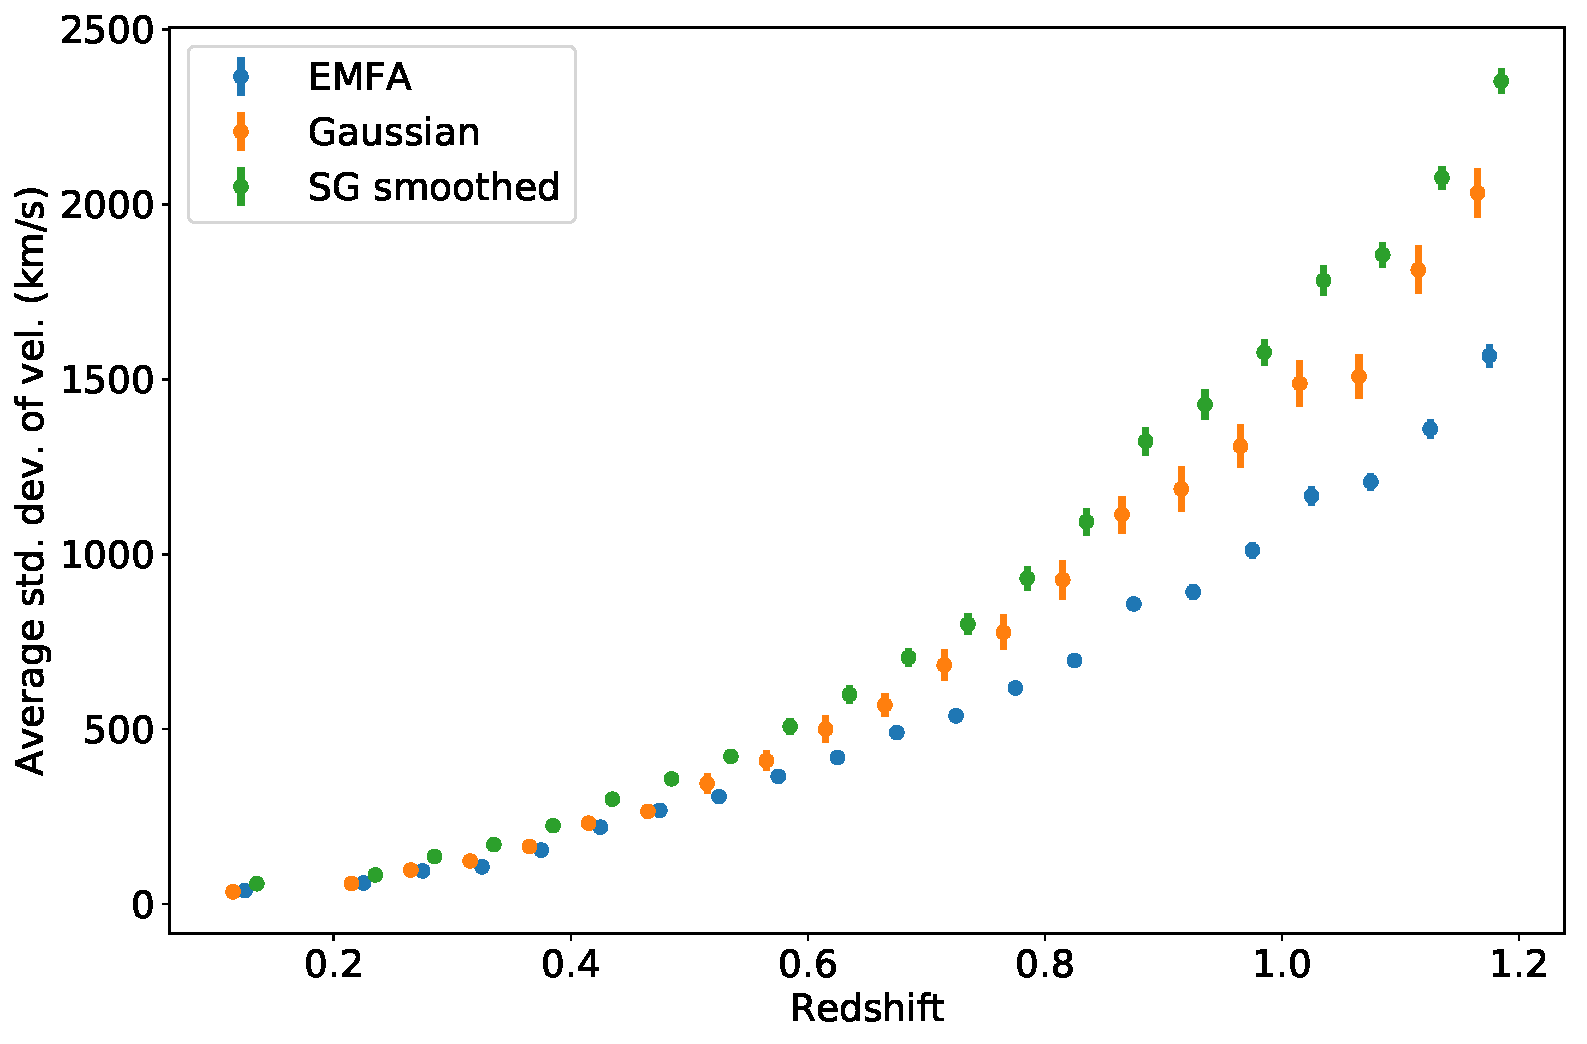
\includegraphics[width=0.9\textwidth]{figures/si_feat_pca/wfirst_vel_uncert.pdf}
    \caption{Per-redshift-bin average of the per-object standard deviations of the velocity measured with three techniques plotted as a function of redshift for the simulated Roman prism spectra. The EMFA recovery technique outperforms both the Gaussian and SG filter smoothing techniques at all redshifts.}
    \label{wfirst_vel_uncertainty_vs_z}
\end{figure}

\begin{figure}[htbp]
    \centering
    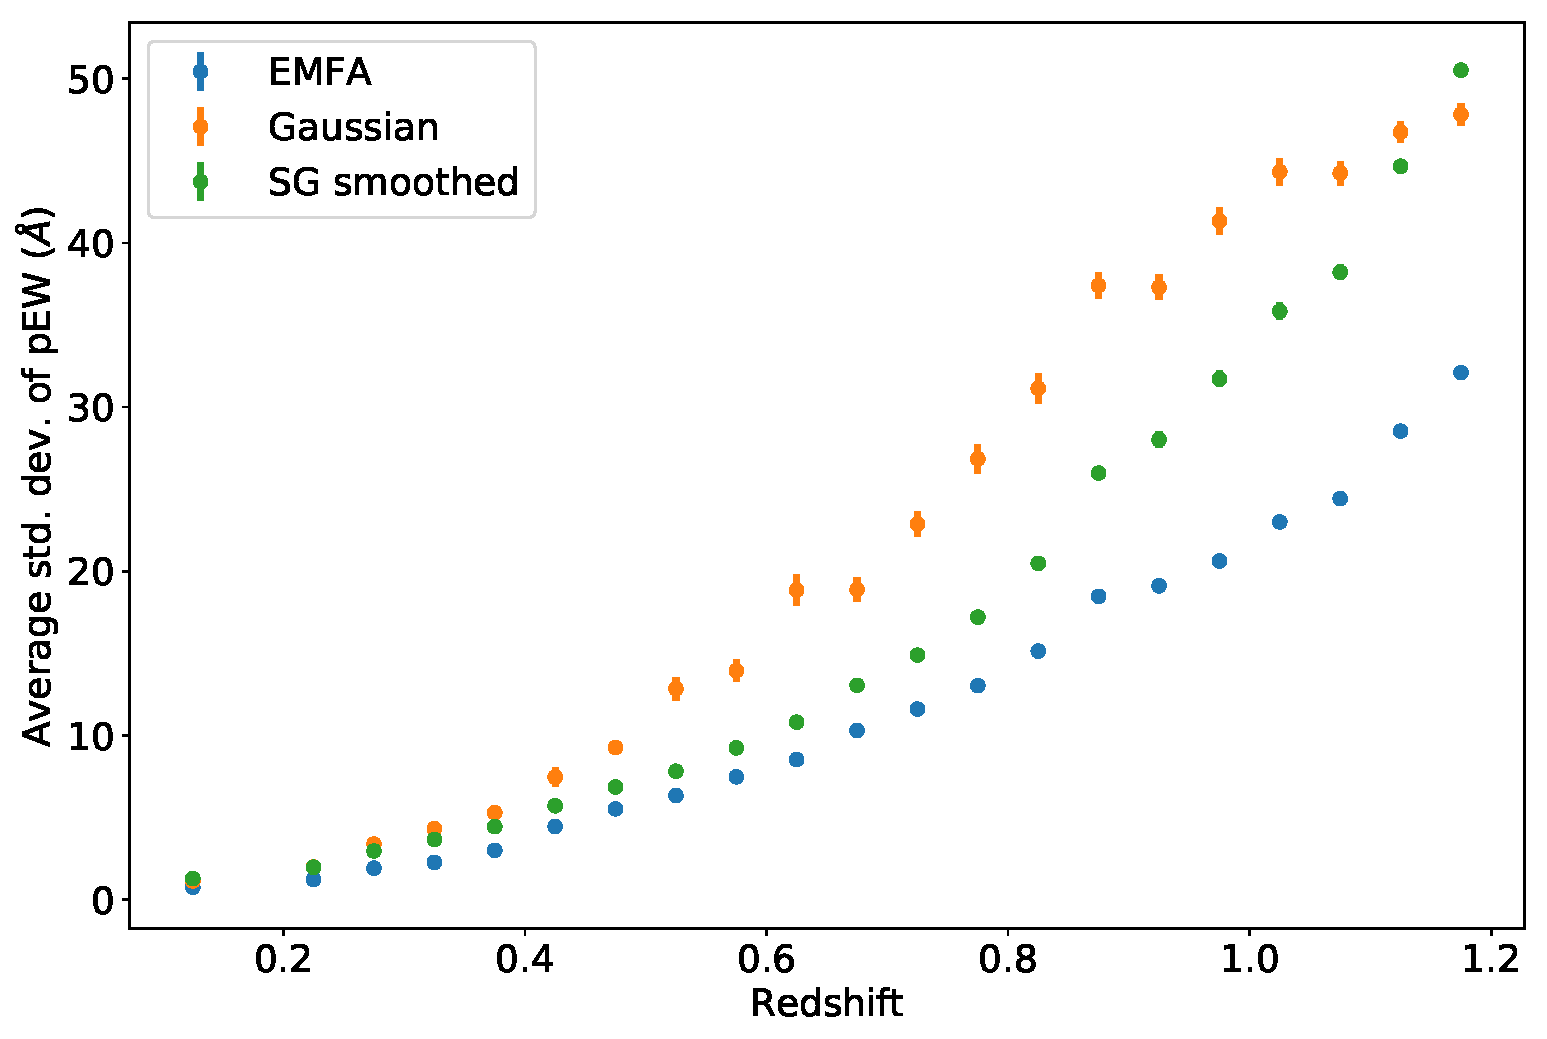
\includegraphics[width=0.9\textwidth]{figures/si_feat_pca/wfirst_pew_uncert.pdf}
    \caption{Same as Figure \ref{wfirst_vel_uncertainty_vs_z}, but for pseudo-equivalent width measurements. In contrast to the velocity measurement uncertainty, the SG filter smoothing methods seems to perform better than the Gaussian measurement in this metric. However, the EMFA still out-performs both methods.}
    \label{wfirst_ew_uncertainty_vs_z}
\end{figure}

From this benchmark prism survey simulation, we find that our new method for recovering the \siliconii{} spectral indicators is both more precise and more accurate than other commonly used measurement techniques. By using a model of the feature informed by the data, we are able to extract more useful information from noisier data, allowing us to obtain the same spectral information in shorter exposure times, or equivalently out to higher redshifts with the same exposure time.

\section{Conclusions}
\label{conclusions}
We have presented a new method for reconstructing the \siliconii{} spectral feature of Type Ia supernovae. By using available high-resolution spectroscopic data, we are able to recover the velocity and equivalent width of the feature in low-resolution, noisy spectra with more precision and accuracy than the other methods shown. We have validated our model on an outside data set to ensure that the model was not overtrained and could generalize to other data sets. We also tested the performance of the model on simulated lower-resolution data for a range of signal-to-noise ratios as a benchmark, finding significant improvements in the measurement uncertainty and systematic error when using this new model instead of other techniques.

The results of the simulations can be used in future work to optimize cadence, observation, and instrument designs for upcoming supernova surveys. The improved performance in this metric could allow for more objects to be observed, or for even more accurate estimates of spectral indicators with the same exposure times. 

% There are several paths to extend this work. In our validation, we saw an example of the failure of the EMFA recovery technique to capture very broad, high-velocity features because of the lack of such examples in the training set. Future iterations of the with a larger and more diverse training set could remedy these types of failures. Another logical extension to this work would be to repeat this analysis for other spectral features (e.g. Ca II H\&K), or to go beyond observations near max and build a model of the temporal evolution of these features. Dixon et al. (in preparation) will continue this generalization, by using SNEMO \citep{saunders_snemo_2018} (an EMFA of full spectral time-series of SNe Ia) to recover a variety of spectral indicators from spectra observed at a range of phases or from photometric measurements.
